\documentclass[11pt]{article}
\usepackage[T1]{fontenc}
\usepackage{lmodern}
\input{glyphtounicode}
\pdfgentounicode=1
\pdfglyphtounicode{braceleftBigg}{007B}
\pdfglyphtounicode{braceleftbig}{007B}
\pdfglyphtounicode{braceleftbt}{23A9}
\pdfglyphtounicode{braceleftmid}{23A8}
\pdfglyphtounicode{bracelefttp}{23A7}
\pdfglyphtounicode{bracerightbig}{007D}
\pdfglyphtounicode{bracerightbt}{23AD}
\pdfglyphtounicode{bracerightmid}{23AC}
\pdfglyphtounicode{bracerighttp}{23AB}
\pdfglyphtounicode{bracketleftbig}{005B}
\pdfglyphtounicode{bracketrightbig}{005D}
\pdfglyphtounicode{ceilingleftBig}{2308}
\pdfglyphtounicode{ceilingleftbigg}{2308}
\pdfglyphtounicode{ceilingrightBig}{2309}
\pdfglyphtounicode{ceilingrightbigg}{2309}
\pdfglyphtounicode{floorleftbigg}{230A}
\pdfglyphtounicode{floorrightbigg}{230B}
\pdfglyphtounicode{parenleftBigg}{0028}
\pdfglyphtounicode{parenleftbig}{0028}
\pdfglyphtounicode{parenleftbigg}{0028}
\pdfglyphtounicode{parenleftbt}{239D}
\pdfglyphtounicode{parenlefttp}{239B}
\pdfglyphtounicode{parenrightBigg}{0029}
\pdfglyphtounicode{parenrightbig}{0029}
\pdfglyphtounicode{parenrightbigg}{0029}
\pdfglyphtounicode{parenrightbt}{23A0}
\pdfglyphtounicode{parenrighttp}{239E}
\pdfglyphtounicode{summationdisplay}{2211}
\pdfglyphtounicode{uniondisplay}{22C3}
\pdfglyphtounicode{uniontext}{22C3}
\pdfglyphtounicode{vextendsingle}{23D0}

\pdfinfoomitdate=1
\pdftrailerid{}
\pdfsuppressptexinfo=15
\usepackage[margin=1in]{geometry}
\usepackage{amsmath,amssymb,amsthm,mathtools}
\usepackage{booktabs,enumitem,graphicx,tikz}
\usetikzlibrary{arrows.meta,positioning,fit,calc,backgrounds}
\usepackage{microtype}
\usepackage[numbers,sort&compress]{natbib}
\usepackage{xurl}
\usepackage[colorlinks=true,linkcolor=blue!45!black,citecolor=blue!45!black,urlcolor=blue!45!black]{hyperref}
\hypersetup{pdftitle={A linear list-coloring bound in terms of the Hadwiger number},pdfauthor={OpenAI},pdfsubject={Linear List Hadwiger conjecture}}
\newtheorem{theorem}{Theorem}[section]
\newtheorem{lemma}[theorem]{Lemma}
\newtheorem{proposition}[theorem]{Proposition}
\newtheorem{corollary}[theorem]{Corollary}
\theoremstyle{definition}
\newtheorem{definition}[theorem]{Definition}
\theoremstyle{remark}
\newtheorem{remark}[theorem]{Remark}
\title{A linear list-coloring bound in terms\\of the Hadwiger number}
\author{OpenAI}
\date{September 23, 2026}
\begin{document}
\maketitle
\begin{abstract}
We prove that every finite nonempty graph $G$ satisfies
$\chi_{\mathrm{list}}(G)\le C h(G)$ for an absolute integer $C$, where
$h(G)$ is the largest order of a clique minor. This resolves the Linear
List Hadwiger conjecture affirmatively.
\end{abstract}
\section{Introduction}\label{sec:introduction}

A clique minor records a form of complete interaction inside a graph:
its vertices are represented by disjoint connected sets, and every two
sets have an edge between them. For a finite nonempty simple graph $G$,
let $h(G)$ be the largest order of a clique minor in $G$. Hadwiger
conjectured that the chromatic number always satisfies
$\chi(G)\le h(G)$ \cite{Hadwiger1943}. The companion manuscript
\cite[Corollary~1.2]{OpenAIHadwigerCounterexample2026} constructs finite
simple graphs with $\chi(G)>h(G)$, disproving this ordinary coefficient-one
assertion. Its linear relaxation asks whether
an absolute constant can replace the coefficient one. We prove a bound
of this form even when allowable colors vary from vertex to vertex.

A \emph{list assignment} $\mathcal L$ assigns a finite set of colors to
each vertex. An $\mathcal L$-coloring is a proper coloring $c$ satisfying
$c(v)\in\mathcal L(v)$ at every vertex. The list chromatic number
$\ell(G)=\chi_{\mathrm{list}}(G)$ is the least integer $k$ for which every
assignment with $|\mathcal L(v)|\ge k$ is colorable. List coloring was
introduced independently by Vizing \cite{Vizing1976} and by Erd\H{o}s,
Rubin, and Taylor \cite{ErdosRubinTaylor1980}. The linear list
version of Hadwiger's conjecture was formulated by Kawarabayashi and
Mohar \cite[Conjecture~1.3]{KawarabayashiMohar2007}.

\begin{theorem}\label{thm:main}
There is an absolute integer $C\ge1$ such that every finite nonempty
simple graph $G$ satisfies
\[
 \ell(G)\le C h(G).
\]
\end{theorem}

Thus the Linear List Hadwiger conjecture has an affirmative resolution.
The constant is independent of the graph order, the list assignment, and
the number of distinct colors appearing in its union. Taking the same
list at every vertex immediately gives the ordinary conclusion.

\begin{corollary}\label{cor:ordinary}
Every finite nonempty simple graph $G$ satisfies $\chi(G)\le C h(G)$,
with the constant $C$ in Theorem~\ref{thm:main}.
\end{corollary}
\begin{proof}
A coloring from the common list $\{1,\ldots,\ell(G)\}$ shows that
$\chi(G)\le\ell(G)$.
\end{proof}

\subsection{Prior work and the two obstacles}

The density theorems of Kostochka \cite{Kostochka1982,Kostochka1984}
and Thomason \cite{Thomason1984} show that every $K_t$-minor-free graph
has a vertex of degree $O(t\sqrt{\log t})$, as does each of its
subgraphs. Greedy coloring in reverse deletion order therefore gives
this bound for arbitrary lists. Norin, Postle, and Song
\cite{NorinPostleSong2023} went beyond that degeneracy threshold for
ordinary coloring, proving $O(t(\log t)^\beta)$ for every fixed
$\beta>1/4$. Norin and Postle \cite{NorinPostle2023} extended such
bounds to list coloring using the structure of highly connected
minor-free graphs.

The coefficient in a linear list bound has a different role from the
coefficient in ordinary Hadwiger's conjecture. Voigt
\cite{Voigt1993} constructed planar graphs that are not $4$-choosable.
Bar\'at, Joret, and Wood \cite{BaratJoretWood2011} constructed graphs
with no $K_{3s+2}$ minor that are not $4s$-choosable for every integer
$s\ge1$, and Steiner
\cite{Steiner2022List} proved that for every $\varepsilon>0$ and all
sufficiently large $t$ there are $K_t$-minor-free graphs with list
chromatic number at least $(2-\varepsilon)t$. Thus a universal constant
in Theorem~\ref{thm:main} must be at least two. Our constants are not
optimized.

The fractional coloring theorem of Reed and Seymour
\cite{ReedSeymour1998} gives $\chi_f(G)\le2h(G)$, where fractional
coloring permits weighted stable sets in place of color classes. It
provides a linear supply of stable sets but does not directly give a
linear ordinary or list coloring: naive repeated sampling introduces a
factor depending on the graph order. Delcourt and Postle
\cite{DelcourtPostle2021} obtained the ordinary bound
$O(t\log\log t)$ for graphs excluding a $K_t$ minor and reduced a linear
ordinary bound to coloring suitably small subgraphs. Liu and Luo
\cite{LiuLuo2026} subsequently proved the ordinary bound
$O(t\log\log\log t)$ and developed bounded stable-set sampling that we
use below.\footnote{Liu and Luo explicitly acknowledge assistance from
ChatGPT Codex; their declaration does not identify an underlying model
version.} These ordinary-coloring statements do not by themselves give
colorings from arbitrary vertex lists.

For list coloring, Postle proved an $O(t(\log\log t)^6)$ bound for
$K_t$-minor-free graphs \cite[Theorem~1.8]{Postle2020}. His separability
and woven-minor constructions provide the structural framework for our
passage from small graphs to arbitrary orders. Delcourt and Postle outlined
an $O(t(\log\log t)^2)$ list bound in the first version of their paper
\cite[Section~6]{DelcourtPostle2021v1}, leaving the details to the reader.
In subsequent work posted on October~1, 2026, Gu and Xu
\cite[Theorem~1.3]{GuXu2026} proved an $O(t\log\log t)$ list bound.
Connectivity extraction by the constraint-budget method of Gir\~ao and Narayanan
\cite{GiraoNarayanan2022}, and the highly linked graph theorem of
Bollob\'as and Thomason \cite{BollobasThomason1996}, are further key
antecedents. We reproduce the list transfer, density, path accounting,
and recursion arguments in the forms required here.

Two difficulties remain after these reductions. Even on a small graph,
a sampled stable set cannot be given a single color unless that color is
available at every vertex receiving it. In a graph of unrestricted order,
the paths used to assemble a minor may themselves contain arbitrarily
many vertices. Their deletion must therefore be charged through their
structure, rather than through their order. The proof addresses these
two difficulties separately.

\subsection{Proof strategy}

First, Proposition~\ref{prop:small-list} proves that a $K_t$-minor-free
graph on at most $t^{11/10}$ vertices is $Lt$-choosable, for an absolute
$L$ and all sufficiently large $t$. We partition the union of all lists
into bins, assigning each color to a single bin throughout the graph.
A vertex is eligible for a bin precisely when its own list contains a
color in that bin. A random partition gives every vertex enough eligible
bins at every stage, before any remaining graph is chosen.
Lemma~\ref{small:eligible-thinning} then repeatedly halves an upper bound
on the fractional chromatic number using sampled stable sets restricted to eligible
vertices. Vertices assigned to the same bin lie in one stable set, so
each can choose its own allowable color from that bin; colors in different
bins cannot conflict.

To prove the thinning lemma, suppose every sampling outcome leaves a
fractional chromatic number greater than half the current bound. A deterministic separator
decomposition finds a fixed highly connected subgraph in which a
remainder still has large expected fractional chromatic number. Independent
repetitions produce disjoint private vertex sets, each supporting a clique
model. A small, fixed family of matching tests shows that the complement
of the union of the sampled remainders remains highly connected.
Connecting equally labeled bags through this complement produces the
excluded clique minor. The proof uses bounded stable-set sampling and
ordinary-chromatic connectivity extraction, with the full argument given
in Section~\ref{small:section}. Summing the costs of successive halving
stages requires only $O(t)$ bins.

Second, Lemma~\ref{lem:list-extraction} extracts highly connected
subgraphs with a linear loss of list chromatic number. The additive
list-deletion estimate, Lemma~\ref{lem:additive-deletion}, reserves
colors for a small set and controls its interaction with all remaining
vertices. Its probabilistic estimate tests only polynomially many
exceptional vertices, independently of the ambient graph order and
palette size. Minimum-length path systems give the sparsity needed to
apply this estimate even when the paths are long. The density argument
also supplies small highly connected subgraphs in which clique models
can be built while connecting paths are rerouted.

The sequential construction in Lemma~\ref{lem:separability} then shows
that a graph of sufficiently large list chromatic number either contains
the desired clique minor or splits into two disjoint subgraphs retaining
nearly all of that list chromatic number. At each step, one small district
supplies new adjacencies between model bags and a separate junction joins
the paths carrying those bags forward. The deletion estimate applies to
the complete history of original minimizing paths, including vertices
no longer used by the growing model.

Finally, Theorem~\ref{thm:recursive-woven} builds a clique model whose
bags contain prescribed roots, together with paths for prescribed
terminal pairs. After reserving the paths for the terminal pairs, the
remaining task is a rooted model inside a fresh region. Separability
supplies three disjoint districts for recursive calls. Partitioning the
root labels into three blocks and assigning one district to each pair
of blocks reduces each call to about two thirds as many roots, while
every pair of labels still occurs together in one district. Connectivity
extraction and the case with no prescribed pairs complete the theorem.

Section~\ref{sec:preliminaries} fixes the external inputs and
probabilistic tools. Section~\ref{small:section} proves the small-graph
list bound, and Section~\ref{sec:list-transfer} establishes list
extraction and deletion. Section~\ref{sec:density} constructs small
highly connected districts; Section~\ref{sec:routing} develops their
routing interfaces. Sections~\ref{sec:separability} and
\ref{sec:recursion} prove separability and the final recursive theorem.
The only structural results used without proof are the fractional minor
bound, ordinary-chromatic connectivity extraction, and the terminal
grouping theorem, whose precise statements follow.

\section{Preliminaries and probabilistic tools}\label{sec:preliminaries}

All graphs are finite, simple, and undirected. A \emph{stable set} is a set
of pairwise nonadjacent vertices. For a vertex set $X$, write $P[X]$ for
the induced subgraph and $P-X=P[V(P)\setminus X]$. A clique model consists
of disjoint nonempty connected vertex sets, called \emph{bags}, with an
edge between every two bags. Models lift through edge contractions and
vertex deletions, so $h$ is nonincreasing under taking minors. Whenever
a subgraph is specified by its vertices, it is induced. Adding edges to
a connected or highly connected subgraph preserves the corresponding
property, so the subgraphs produced below may be replaced by induced
subgraphs on their vertices.

A graph is $k$-connected if it has more than $k$ vertices and remains
connected after deletion of fewer than $k$ vertices. Such a graph has
minimum degree at least $k$. A separator split is a partition
$V(P)=A\mathbin{\dot\cup}Z\mathbin{\dot\cup}A'$, with $A,A'$ nonempty
and anticomplete. If $|V(P)|>k$ and $P$ is not $k$-connected, there is such
a split with $|Z|<k$. Deleting $z<k$ vertices from a $k$-connected graph
leaves a $(k-z)$-connected graph. All logarithms are natural. The null
graph has $h=\ell=\chi=f=0$. Integer parameters include minor orders,
connectivity requirements, and numbers of paths; powers bounding graph
orders need not be integers.

\subsection{Fractional coloring and established structural results}

The fractional chromatic number $f(P)$ is the minimum total weight of
nonnegative weights on the stable sets of $P$ that cover every vertex
with weight at least one. Finite linear-programming duality
\cite{galekuhntucker1951} gives
\begin{equation}\label{eq:fractional-dual}
 f(P)=\max\left\{\sum_{v\in V(P)}w(v):
 w(v)\ge0,\quad \sum_{v\in I}w(v)\le1
 \text{ for every stable set }I\right\}.
\end{equation}
The primal is feasible, using singleton stable sets, and has a finite
optimum; thus this use of duality has no feasibility or boundedness
exception. For $r>0$, $f(P)\le r$ is equivalent to a distribution on stable
sets with every vertex included with probability at least $1/r$.
Indeed, divide a fractional coloring by $r$ and put any missing mass on
the empty set; conversely multiply such a distribution by $r$.
Restriction to an induced subgraph cannot increase $f$, and adding one
vertex increases it by at most one.

\begin{theorem}[Fractional minor bound]\label{thm:fractional}
Every graph $P$ satisfies $f(P)\le4h(P)$.
\end{theorem}
This follows from the stronger bound $f(P)\le2h(P)$ of Reed and Seymour
\cite[Statement~(1.3)]{ReedSeymour1998}. We keep the factor four throughout.

\begin{theorem}[Ordinary-chromatic connectivity extraction]
\label{thm:ordinary-extraction}
If $k\ge1$ is an integer and $\chi(P)\ge7k$, then $P$ has a
$k$-connected subgraph $J$ with $\chi(J)\ge\chi(P)-6k$.
\end{theorem}
We use the form stated in \cite[Theorem~5.1]{DelcourtPostle2021},
attributed there to Gir\~ao and Narayanan. There is no minor-exclusion
hypothesis. In particular the theorem applies to auxiliary clique
blow-ups, which need not inherit any minor exclusion.

\begin{theorem}[Grouping terminals]\label{thm:grouping}
There is an absolute integer $\gamma\ge1$ such that the following holds.
In a $\gamma m$-connected graph, every partition of $m\ge1$ distinct
terminals into nonempty groups can be realized by pairwise disjoint
connected vertex sets, one containing each group.
\end{theorem}
This is a consequence of the highly linked graph theorem of
Bollob\'as and Thomason \cite{BollobasThomason1996}; we use the
case with second knitting parameter one in
\cite[Definition~5.7 and Theorem~5.8]{DelcourtPostle2021}. The constant
$\gamma$ is uniform in the number and sizes of the groups. For a group
of size two, a path within its connected set joins its terminals. We
will apply this observation to any prescribed pairing of distinct
terminals.

\subsection{Bounded sampling and concentration}

The following real-parameter form of bounded stable-set sampling is
convenient. Its integer-parameter form appears in
\cite[Lemma~4.1]{LiuLuo2026}; we include the short proof.

\begin{lemma}\label{lem:bounded}
Suppose $|V(P)|\le n$, where $n\ge1$, and $f(P)\le r$, where $r\ge1$.
There is a distribution on stable sets $I$ such that
\[
 |I|\le\lceil n/r\rceil,
 \qquad \Pr(v\in I)=\frac1{2r}\quad(v\in V(P)).
\]
\end{lemma}
\begin{proof}
Start with a stable-set distribution having inclusion probabilities at
least $1/r$. Conditional independent deletion of each included vertex
reduces every marginal to exactly $1/r$ and preserves stability.
Put $M=\lceil n/r\rceil$. Partition each resulting stable set $I$ into
parts of size at most $M$, assigning its probability mass to each part.
This gives a finite measure of total mass at most
\[
 \mathbb E\bigl(1+|I|/M\bigr)
 =1+|V(P)|/(rM)\le2.
\]
Every vertex still has mass $1/r$. Add mass on the empty set to make the
total exactly two and divide by two.
\end{proof}

We also record the standard bounded-martingale-difference estimate
\cite{azuma1967,mcdiarmid1989}, with its short exponential-moment proof.

\begin{lemma}[Bounded differences]\label{lem:concentration}
Let $Z$ be a function of $s\ge1$ independent finite random variables.
If changing one variable changes $Z$ by at most $b>0$, then
\[
 \Pr\bigl(|Z-\mathbb EZ|\ge u\bigr)
 \le2\exp\bigl(-u^2/(2sb^2)\bigr)\qquad(u>0).
\]
\end{lemma}
\begin{proof}
Expose the variables in order. The martingale of conditional
expectations has differences of conditional mean zero and absolute
value at most $b$. Convexity bounds the conditional exponential moment
of a difference at $\lambda$ by
$\cosh(\lambda b)\le\exp(\lambda^2b^2/2)$.
Multiplying these bounds and applying Markov's inequality with
$\lambda=u/(sb^2)$ gives the upper tail. Apply the same argument to $-Z$
and add the two bounds.
\end{proof}

\subsection{A small family of connectivity tests}

The next test replaces an enumeration of arbitrary vertex cuts by an
enumeration of unions of a few open neighborhoods. The family is fixed
before the random deleted set is chosen.

\begin{lemma}[Cut test]\label{lem:cut-test}
Let $P$ be a $k$-connected graph on at most $n$ vertices, where $k$ is a
sufficiently large integer. Set
\[
 s=\left\lceil10(n/k)\log(2n)\right\rceil.
\]
There is a family of at most $(n+1)^{s+1}$ matchings, each of size
$\lfloor k/8\rfloor$, with the following property. If $U\subseteq V(P)$,
every vertex of $P$ has at least $k/2$ neighbors outside $U$, and fewer
than $k/32$ endpoints of each matching belong to $U$, then $P-U$ is
$\lfloor k/32\rfloor$-connected.
\end{lemma}
\begin{proof}
For every set $R$ of at most $s$ vertices, put
$B_R=\bigcup_{v\in R}N_P(v)$. Whenever both $B_R$ and its complement
have size at least $k/3$, fix a matching of size $\lfloor k/8\rfloor$
across this cut. Such a matching exists: otherwise the endpoints of a
maximal smaller matching form a vertex cover of the crossing edges,
of size less than $k/4$. Both sides remain nonempty after their removal,
contradicting $k$-connectivity. The number of possible sets $R$, and
hence of matchings, is at most $(n+1)^{s+1}$.

The neighborhood assumption ensures that $P-U$ has more than
$\lfloor k/32\rfloor$ vertices. If it fails the asserted connectivity,
there are a set $Z\subseteq V(P)\setminus U$ with $|Z|<k/32$ and
nonempty anticomplete sides $A,A'$ partitioning $V(P)\setminus(U\cup Z)$.
Every vertex of either side has more than $k/3$ neighbors in that same
side, since it has at least $k/2$ neighbors outside $U$ and loses fewer
than $k/32$ to $Z$. In particular both sides have size at least $k/3$.

Make $s$ independent uniform draws from $A$. For each vertex $v\in A$,
the probability that none of the draws is an open neighbor of $v$ is
at most $\exp(-ks/(3n))$. The union bound over $A$ is less than one by
the choice of $s$. Thus the set $R$ of drawn vertices, after repetitions
are removed, satisfies $A\subseteq B_R$. Since $A,A'$ are anticomplete,
$A'\cap B_R=\varnothing$. The matching fixed for this cut has every edge
incident with $U\cup Z$, for otherwise an edge would join $A$ to $A'$.
But $U$ contains fewer than $k/32$ of its endpoints, and $Z$ contains
fewer than $k/32$ vertices. They cannot cover its
$\lfloor k/8\rfloor$ disjoint edges. This contradiction proves the
lemma.
\end{proof}

\section{List coloring small graphs}
\label{small:section}

\begin{proposition}\label{prop:small-list}
There are an absolute positive integer $L$ and an absolute integer $t_0$
such that, for every integer $t\ge t_0$ and every graph $G$,
\[
 h(G)<t,\qquad |V(G)|\le t^{11/10}
 \quad\Longrightarrow\quad \ell(G)\le Lt.
\]
\end{proposition}

We will color the graph in stages, halving an upper bound on its fractional
chromatic number at each stage. For each sampled stable set, only a specified
subset of vertices is eligible to be removed. The next lemma allows
these eligibility restrictions to be fixed in advance. In the final
application they will come from one partition of the actual colors
appearing in the lists, chosen before the successive remaining graphs
are determined.

\begin{lemma}[Eligible thinning]\label{small:eligible-thinning}
There is an absolute positive integer $B$ such that the following holds
for all sufficiently large integers $t$. Let $n,r$ be real parameters with
\[
 1\le n\le t^{11/10},\qquad \frac{t}{\log t}\le r\le4t,
\]
and let $P$ be a graph with $|V(P)|\le n$, $h(P)<t$, and $f(P)\le r$.
Set
\[
 N=\left\lceil Br\log\bigl(2\max\{1,t/r\}\bigr)\right\rceil.
\]
Suppose $E_1,\ldots,E_N\subseteq V(P)$ contain every vertex at least
$N/2$ times. There are stable sets $I_1,\ldots,I_N$ of $P$, each of size
at most $\lceil n/r\rceil$, such that
\[
 f\left(P-\bigcup_{j=1}^N(I_j\cap E_j)\right)\le r/2.
\]
The cutoff for $t$ is uniform over $P,n,r$ and the eligibility sets.
\end{lemma}

We prove the lemma by contradiction. If every sampled remainder has
fractional chromatic number greater than $r/2$, we first find a fixed
highly connected subgraph $H$ where a remainder still has large expected
fractional chromatic number. Fresh independent remainders then contain
disjoint subsets, each carrying a clique model. The complement in $H$
of the union of the remainders remains highly connected. To assemble a
$K_t$ model, partition its $t$ labels into small blocks and use one of
these disjoint models for each
block and each pair of blocks. The complement connects all bags assigned
to the same label. Every pair of labels is represented together in one
model, so the resulting label sets are adjacent. The estimates below
provide the models and the connectivity for this construction.

\subsection{Eligible samples and uniform concentration}

We prove Lemma~\ref{small:eligible-thinning} with the following fixed
choice of $B$. Let $\gamma$ be the integer in
Theorem~\ref{thm:grouping}. Fix
\begin{equation}\label{small:constants}
 D_0=10^6\gamma,\qquad Q_0=401^2,
\end{equation}
and choose a positive integer $B$ such that
\begin{equation}\label{small:B-choice}
 B\ge16,\qquad
 2^{B/4}\ge
 \max\bigl\{2000(D_0+1),\,10^4Q_0^2\bigr\}.
\end{equation}
These constants remain fixed throughout this section.

Consider an integer $t$ and real parameters $n,r$ satisfying
\begin{equation}\label{small:range}
 1\le n\le t^{11/10},\qquad
 \frac{t}{\log t}\le r\le4t.
\end{equation}
Let $P$ be a graph on at most $n$ vertices with $h(P)<t$ and $f(P)\le r$.
Set
\begin{equation}\label{small:parameters}
 \begin{gathered}
 y=\max\{1,t/r\},\qquad x=\lfloor r/200\rfloor,
 \qquad q=\lceil t/x\rceil^2,\qquad k=\lceil D_0ty\rceil,\\
 N=\lceil Br\log(2y)\rceil,\qquad M=\lceil n/r\rceil.
 \end{gathered}
\end{equation}
Here $x$ bounds the size of a label block, $q$ bounds the number of
disjoint clique models, and $k$ is the connectivity required of $H$.
The parameters $N$ and $M$ are the number of trials and the maximum
size of one sampled stable set.
We always take $t$ above an absolute cutoff large enough that $r\ge400$.
In particular $x\ge1$. The following bounds hold uniformly in
\eqref{small:range}:
\begin{equation}\label{small:parameter-bounds}
 \begin{gathered}
 1\le y\le\log t,\qquad \frac{t}{y}\le r\le\frac{4t}{y},\qquad
 x\ge\frac r{400},\\
 q\le Q_0y^2,\qquad xq\le403ty,\qquad
 D_0ty\le k\le(D_0+1)ty.
 \end{gathered}
\end{equation}
Indeed, $t/x\le400t/r\le400y$, so
$\lceil t/x\rceil\le401y$. Also
\[
 x\lceil t/x\rceil^2
 \le\frac{t^2}{x}+2t+x
 \le400\frac{t^2}{r}+2t+\frac r{200}
 \le403ty.
\]
Our choice of $D_0$ consequently gives, for all sufficiently large $t$,
\begin{equation}\label{small:attachment-budget}
 k\ge r,\qquad 2xq<\frac{k}{64},\qquad
 \left\lfloor\frac{k}{32}\right\rfloor\ge\gamma(2xq).
\end{equation}

Fix sets $E_1,\ldots,E_N\subseteq V(P)$ such that each vertex belongs
to at least $N/2$ of them. These are the eligibility sets and are fixed
before sampling. Independently for each $j\in\{1,\ldots,N\}$, sample a
stable set $I_j$ from the distribution in Lemma~\ref{lem:bounded}, with
\[
 |I_j|\le M,\qquad \Pr(v\in I_j)=\frac1{2r}.
\]
The covered vertices at trial $j$ are $I_j\cap E_j$, and the remainder is
\begin{equation}\label{small:remainder}
 W=V(P)\setminus\bigcup_{j=1}^N(I_j\cap E_j).
\end{equation}
For every vertex $v$, independence of the trials and the eligibility
condition imply
\begin{equation}\label{small:survival}
 \Pr(v\in W)
 \le\left(1-\frac1{2r}\right)^{N/2}
 \le p:=\exp\left(-\frac{N}{4r}\right)
 \le(2y)^{-B/4}.
\end{equation}
In particular, \eqref{small:B-choice} and \eqref{small:parameter-bounds}
give
\begin{equation}\label{small:sparseness}
 2kp\le\frac r{1000},\qquad q^2p\le10^{-4}.
\end{equation}
For the first inequality, divide by $r$ and use
\[
 \frac{2kp}{r}
 \le2(D_0+1)y^2(2y)^{-B/4}
 \le2(D_0+1)2^{-B/4}.
\]
For the second, use
$q^2p\le Q_0^2y^4(2y)^{-B/4}\le Q_0^2 2^{-B/4}$.

\begin{lemma}\label{small:concentration}
Take at most $q$ independent copies of the experiment
\eqref{small:remainder}. Let $Z$ be any one of the following quantities,
where the vertex set $A\subseteq V(P)$ is fixed before sampling:
\[
 |A\cap W_i|,\qquad
 \left|A\cap\bigcup_iW_i\right|,\qquad
 f(P[A\cap W_i]).
\]
For each fixed $\delta>0$, and all sufficiently large $t$,
\begin{equation}\label{small:uniform-tail}
 \Pr\bigl(|Z-\mathbb EZ|\ge\delta r\bigr)
 \le2\exp(-t^{7/10}),
\end{equation}
uniformly over all the data in \eqref{small:range} and all eligibility
sets satisfying the stated condition.
\end{lemma}

\begin{proof}
Changing one sampled stable set changes $W_i$ on at most $2M$ vertices.
It changes a union of remainders on at most the same number of vertices.
Adding or deleting a vertex changes fractional chromatic number by at
most one, so all the quantities in the statement have bounded differences
at most $2M$ per trial.

For sufficiently large $t$, $r\log(2y)\ge1$, and hence
$N\le(B+1)r\log(2y)$. With
$A_0=4Q_0(B+1)$, we obtain
\[
 qN\le A_0ty\log(2y),\qquad M\le2t^{1/10}y.
\]
Lemma~\ref{lem:concentration} therefore gives
\begin{align*}
 \Pr\bigl(|Z-\mathbb EZ|\ge\delta r\bigr)
 &\le2\exp\left(-\frac{\delta^2r^2}{2(qN)(2M)^2}\right)\\
 &\le2\exp\left(
 -\frac{\delta^2t^{4/5}}{32A_0y^5\log(2y)}\right).
\end{align*}
Since $1\le y\le\log t$, the exponent in the last line has magnitude at
least $t^{7/10}$ for all sufficiently large $t$. The cutoff depends only
on $\delta$ and the fixed constants. Independence between different
vertices is not used.
\end{proof}

All asymptotic probability estimates below are uniform over these data.
Only finitely many fixed positive values of $\delta$ will be used in
Lemma~\ref{small:concentration}, so their cutoffs can be combined.

\subsection{Localizing a failure of thinning}

\begin{lemma}\label{small:fixed-region}
Suppose that every outcome of the experiment
\eqref{small:remainder} having positive probability satisfies
$f(P[W])>r/2$. Then there is a fixed induced $k$-connected subgraph
$H\subseteq P$ such that
\begin{equation}\label{small:region-expectation}
 \mathbb E f(H[W\cap V(H)])>r/4.
\end{equation}
The subgraph $H$ is chosen before any fresh copies of the experiment
are sampled.
\end{lemma}

\begin{proof}
Build a binary decomposition of $P$, making all choices before sampling.
A node is an induced subgraph. Stop at a node of order at most $2k$, and
also at a larger node which is $k$-connected. Otherwise choose a separator
of size less than $k$, partition the vertices outside it into two
nonempty anticomplete sides, and form two children by adding the
separator to each side.

There are $O(n^2+1)$ nodes. To see this, give a node of order $u>2k$
potential $u-k$. Each large child's potential is strictly smaller than
its parent's, since the other exclusive side is nonempty. If both
children are large, their potentials sum to at most their parent's:
their orders sum to $u+|S|<u+k$, where $S$ is the separator. If just one
child is large, its potential alone is at most the parent's. Thus at
each depth the sum of the large-node potentials is at most $n$, while
the depth of a large-node branch is at most $n$. The small leaves
contribute at most two children per large node, in addition to a possible
small root.

Every separator and every small leaf has order at most $2k$. Its expected
intersection size with $W$ is at most $2kp\le r/1000$.
Lemma~\ref{small:concentration} and a union bound over the decomposition
show that, with probability $1-o(1)$, all these intersections have fewer
than $r/100$ vertices. If every $k$-connected leaf had expected fractional
chromatic number at most $r/4$ after restriction to $W$, the same lemma
would give, again with probability $1-o(1)$, fractional chromatic number
less than $3r/10$ in every such leaf. A small leaf has this latter bound
as well, since its fractional chromatic number is at most its order.

Fix an outcome satisfying all these conclusions. Write $F=P[W]$.
The assumption of the lemma gives $f(F)>r/2$, whereas every leaf
restriction has fractional chromatic number less than $3r/10$.
We compare these bounds by replacing every vertex of $F$ with a clique
of the same large order. Ordinary-chromatic connectivity extraction in
this larger graph will produce a subgraph of large chromatic number that
cannot cross any of the blown-up separators. It must lie in one
blown-up leaf, giving the contradiction.

For a positive integer $m$, form $F^{(m)}$ by replacing each vertex of
$F$ with a clique of order $m$, and replacing each edge with a complete
join between its two replacement cliques. Every color class of $F^{(m)}$ projects to a stable
set of $F$ and uses at most one vertex of each replacement clique.
Dividing the multiplicities of these projected stable sets by $m$
therefore gives a fractional coloring of $F$. Consequently
\begin{equation}\label{small:blowup-lower}
 \chi(F^{(m)})\ge mf(F)>mr/2.
\end{equation}

For each leaf restriction, choose a fractional coloring of weight less
than $3r/10$. Round its finitely many stable-set weights up to multiples
of $1/m$. Give a distinct color slot to each unit of weight $1/m$.
Every original vertex belongs to at least $m$ slots, so its $m$ copies
can be assigned distinct slots containing that vertex. A slot is a
stable set upstairs: it contains at most one copy of any original
vertex, and its original vertices form a stable set. The rounding adds
only a bounded number of slots, independent of $m$ for this fixed leaf.
There are finitely many leaves, so for all sufficiently large $m$, every
blown-up leaf restriction has a coloring with fewer than $31mr/100$
colors.

Apply Theorem~\ref{thm:ordinary-extraction} to $F^{(m)}$ with the integer
parameter $k'=\lceil mr/50\rceil$. For sufficiently large $m$,
\eqref{small:blowup-lower} exceeds $7k'$. We obtain a $k'$-connected
subgraph $J$ with
\[
 \chi(J)\ge\chi(F^{(m)})-6k'
 >\frac{19mr}{50}-6
 >\frac{31mr}{100}.
\]
Each restricted separator of the decomposition has fewer than $r/100$
vertices, so its blow-up has fewer than $mr/100<k'$ vertices. Thus $J$
cannot meet both exclusive sides of any such split: deleting its
vertices in the separator would disconnect $J$ with fewer than $k'$
deletions. Nor can $J$ be contained in the separator, because its order
is greater than $k'$. Descending the decomposition places $J$ inside a
single blown-up leaf restriction, contradicting that leaf's coloring
bound.

It follows that some $k$-connected leaf satisfies
\eqref{small:region-expectation}. This argument also covers the case
where $P$ is too small to be $k$-connected: if all leaves were small, the
same contradiction would apply. Finally, the blow-up is only an
auxiliary graph for the extraction theorem, which requires no minor
exclusion; no bound on its clique-minor number was used.
\end{proof}

\subsection{Private models and a connected complement}

Assume the failure hypothesis of Lemma~\ref{small:fixed-region}, and fix
the resulting subgraph $H$. Sample $q$ fresh independent copies
$W_1,\ldots,W_q$ of \eqref{small:remainder}. Put
\[
 T_i=V(H)\cap\left(W_i\setminus\bigcup_{j\ne i}W_j\right),
 \qquad
 U=V(H)\cap\bigcup_{i=1}^qW_i.
\]
The sets $T_i$ are pairwise disjoint subsets of $U$.

\begin{lemma}\label{small:private}
With failure probability at most $4q(q-1)p+o(1)$, every $H[T_i]$ has
fractional chromatic number greater than $r/8$, and hence contains a
$K_{2x}$ model.
\end{lemma}

\begin{proof}
By \eqref{small:region-expectation} and
Lemma~\ref{small:concentration}, the events
\[
 \mathcal A_i=\{f(H[W_i\cap V(H)])>r/5\}
\]
all hold with probability $1-o(1)$: the individual failure probability
is at most $2\exp(-t^{7/10})$, and $q\le Q_0(\log t)^2$.

For each outcome of $W_i$ satisfying $\mathcal A_i$, choose optimal dual
weights on $H[W_i\cap V(H)]$ of total weight $a_i>r/5$.
Choose these weights as a function of $W_i$ alone. Conditional on this
one copy, each other copy still satisfies the vertex survival bound
\eqref{small:survival}. Therefore the expected weight on vertices
belonging to some other copy is at most $(q-1)pa_i$. Markov's inequality
shows that the probability of $\mathcal A_i$ together with the loss of
more than $a_i/4$ is at most $4(q-1)p$.

Taking a union bound over $i$, we conclude that, except with probability
$4q(q-1)p+o(1)$, all private sets retain weight at least
$3a_i/4>3r/20>r/8$. Restriction to $T_i$ preserves dual feasibility:
each stable set in $H[T_i]$ is also a stable set in
$H[W_i\cap V(H)]$. Hence $f(H[T_i])>r/8$. In this calculation we have
conditioned only on a single copy at a time, not on the simultaneous
events $\mathcal A_1,\ldots,\mathcal A_q$.

Theorem~\ref{thm:fractional} now gives
\[
 h(H[T_i])>r/32>2\lfloor r/200\rfloor=2x,
\]
so each private set contains the required model. The models are
vertex-disjoint because the private sets are disjoint.
\end{proof}

\begin{lemma}\label{small:complement}
With probability $1-o(1)$, every vertex of $H$ has at least $k/2$
neighbors in $H-U$, and $H-U$ is $\lfloor k/32\rfloor$-connected.
\end{lemma}

\begin{proof}
Each fixed vertex belongs to $U$ with probability at most
$qp\le10^{-4}$ by \eqref{small:sparseness}. Before sampling, fix $k$
neighbors of each vertex of $H$, possible since $H$ is $k$-connected.
The expected number of those neighbors in $U$ is at most $k/10000$.
Having at least $k/2$ of them in $U$ thus requires a deviation greater
than $k/3\ge r/3$. Lemma~\ref{small:concentration} and a union bound
over at most $n$ vertices prove the neighborhood assertion with
probability $1-o(1)$. This assertion holds for all vertices of $H$,
including those in $U$.

For the connectivity assertion, use the family of test matchings in
Lemma~\ref{lem:cut-test} for the fixed graph $H$, with order bound $n$
and connectivity parameter $k$. Fix this family before sampling the
fresh copies, and set
\[
 s=\left\lceil10\frac nk\log(2n)\right\rceil.
\]
The number of tests is at most
\begin{align*}
 (n+1)^{s+1}
 &=\exp\bigl(O((1+n/k)\log^2(2n))\bigr)\\
 &\le\exp\bigl(O(t^{1/10}\log^2t)\bigr).
\end{align*}
Here the constants are absolute, since $D_0$ is fixed.

The endpoint set of each test matching is a fixed set to which
Lemma~\ref{small:concentration} applies. It has size at most $k/4$, so
its expected intersection size with $U$ is at most $k/40000$. A count of
at least $k/32$ therefore requires a deviation greater than
$k/64\ge r/64$. Lemma~\ref{small:concentration} and the displayed bound
on the number of tests show that, with probability $1-o(1)$, every test
matching has fewer than $k/32$ endpoints in $U$. Together with the
neighborhood assertion, these are the hypotheses of
Lemma~\ref{lem:cut-test}, which gives the claimed connectivity.
\end{proof}

\begin{proof}[Proof of Lemma~\ref{small:eligible-thinning}]
If $P$ is empty, take all the stable sets empty. Otherwise use the
experiment \eqref{small:remainder} and suppose that every outcome of
positive probability has $f(P[W])>r/2$.
Lemma~\ref{small:fixed-region} supplies a fixed $H$. By
\eqref{small:sparseness}, the failure probability in
Lemma~\ref{small:private} is at most $4\cdot10^{-4}+o(1)$.
Thus Lemmas~\ref{small:private} and~\ref{small:complement} hold
simultaneously with positive probability for sufficiently large $t$.
Fix such an outcome, including its $q$ disjoint $K_{2x}$ models.

Partition the $t$ labels of a prospective $K_t$ model into
$b=\lceil t/x\rceil$ nonempty blocks of size at most $x$. Assign a
different private model to each single block and each unordered pair
of distinct blocks. There are
$b+\binom b2=b(b+1)/2\le b^2=q$ assignments. In a model assigned to
one block, retain one bag for each label of that block. In a model
assigned to two blocks, retain one bag for each label in their union.
At most $2x$ bags are retained from each model, and every pair of
distinct labels appears together in one assigned model.

Choose a port vertex in every retained bag. There are at most $2xq$
ports, and each has at least $k/2$ neighbors in $H-U$. By
\eqref{small:attachment-budget}, we can choose a distinct such neighbor
for every port, greedily. Let $m$ be the actual number of chosen
neighbors, so $1\le m\le2xq$. Their labels partition them into $t$
nonempty groups. The graph $H-U$ has connectivity at least
\[
 \left\lfloor\frac{k}{32}\right\rfloor
 \ge\gamma(2xq)\ge\gamma m,
\]
so Theorem~\ref{thm:grouping} provides pairwise disjoint connected sets
in $H-U$ containing these groups.

For each label, unite its connected set in $H-U$ with all its assigned
private bags and their port edges. This set is nonempty and connected.
Different labels give disjoint sets: their connected sets in $H-U$
are disjoint, all private bags are disjoint, and the bags lie in $U$.
Every two label sets are adjacent because their labels occur together
in an assigned clique model. These sets form a $K_t$ model in $P$,
contrary to $h(P)<t$. Some outcome of the sampling experiment must
therefore have fractional chromatic number at most $r/2$, as required.
\end{proof}

\subsection{Assigning the colors to bins}

\begin{proof}[Proof of Proposition~\ref{prop:small-list}]
Fix a sufficiently large integer $t$, and let $G$ satisfy the hypotheses
of the proposition. The empty graph needs no colors, so suppose that
$G$ is nonempty. Set
\[
 r_j=4t2^{-j},\qquad y_j=\max\{1,t/r_j\},
\]
and let $J$ be the largest nonnegative integer for which
$r_J\ge t/\log t$. For each $j\in\{0,\ldots,J\}$, allocate a separate
block of
\[
 N_j=\lceil Br_j\log(2y_j)\rceil
\]
bins. Allocate a further $16t$ bins for cleanup. All these bins are
distinct. Their total number $n_{\mathrm{bin}}$ is at most a fixed
constant times $t$. Indeed, $y_j\le2^j$, so
\begin{align*}
 n_{\mathrm{bin}}
 &\le4Bt\log2\sum_{j\ge0}(j+1)2^{-j}+(J+1)+16t\\
 &=16B(\log2)t+(J+1)+16t.
\end{align*}
Also $J+1=O(\log\log t)$, since $2^J\le4\log t$.
Choose an integer
\[
 D_{\mathrm{bin}}\ge16B\log2+18.
\]
For all sufficiently large $t$, we have
$n_{\mathrm{bin}}\le D_{\mathrm{bin}}t$.
Finally choose a positive integer $L$ such that
\begin{equation}\label{small:L-choice}
 \frac{L}{2D_{\mathrm{bin}}}>\log2+1.
\end{equation}

Let $\mathcal L$ be any finite list assignment on $G$ with
$|\mathcal L(v)|\ge Lt$ at every vertex. Map each color in the finite
union $\bigcup_v\mathcal L(v)$ independently and uniformly to one of
the $n_{\mathrm{bin}}$ bins. We claim that a map can be fixed such that
every vertex has an allowable color in at least half the bins of
every block, including cleanup.

For a fixed vertex and a block of $u$ bins, failure of this property
implies that a subset of $\lceil u/2\rceil$ bins is missed by its list.
For a specified such subset, the probability of being missed is at most
\[
 \left(1-\frac{u}{2n_{\mathrm{bin}}}\right)^{|\mathcal L(v)|}
 \le\exp\left(-\frac{Lt\,u}{2n_{\mathrm{bin}}}\right)
 \le\exp\left(-\frac{Lu}{2D_{\mathrm{bin}}}\right).
\]
There are at most $2^u$ choices for the missed subset, so
\eqref{small:L-choice} bounds the failure probability by $e^{-u}$.
Every nonfinal block has
$u\ge B(\log2)t/\log t$, and the cleanup block has $u=16t$.
Thus, with $c_B=\min\{B\log2,16\}>0$ and $\log t\ge1$, a union bound
over all vertices and blocks gives failure probability at most
\[
 (J+2)t^{11/10}\exp\left(-\frac{c_Bt}{\log t}\right)=o(1).
\]
For sufficiently large $t$, the desired map therefore exists; fix one.
This probability estimate depends on the list sizes, but not on the
number of distinct colors in their union.

Call a vertex eligible for a bin if its list has a color assigned to
that bin. It remains eligible whenever it survives to a later stage.
At the start, Theorem~\ref{thm:fractional} gives $f(G)\le4t=r_0$.
At stage $j$, let $P$ be the current induced remainder. If it is empty,
stop. Otherwise $h(P)<t$, $|V(P)|\le t^{11/10}$, and inductively
$f(P)\le r_j$. For each bin of that stage, take its eligible vertex set
inside $P$. Every vertex belongs to at least half these sets.
Lemma~\ref{small:eligible-thinning}, with $n=t^{11/10}$, supplies a
stable set for each bin such that deleting the eligible covered
vertices leaves fractional chromatic number at most
$r_j/2=r_{j+1}$. Retain one covering bin for every vertex removed at
this stage.

After stage $J$, the remaining graph has fractional chromatic number
at most $r_{J+1}<t/\log t$. If it is nonempty, put $\rho=t/\log t$ and
independently sample a stable set in each cleanup bin from a fractional
coloring distribution having every vertex inclusion probability at
least $1/\rho$. Such a distribution exists because $f\le\rho$.
Every remaining vertex is eligible in at least $8t$ cleanup bins, so
its probability of being missed by all eligible samples is at most
\[
 (1-1/\rho)^{8t}\le\exp(-8t/\rho)=t^{-8}.
\]
The probability that any remaining vertex is missed is therefore at
most $t^{11/10}t^{-8}=t^{-69/10}<1$. Choose an outcome covering every
remaining vertex and again retain one covering bin for each vertex.

Every vertex now has a retained bin and belongs to the stable set
associated with that bin. Choose any color in its original list which
maps to that bin. If two vertices receive the same color, the global
map sends that color to their common retained bin. Both vertices lie
in that bin's stable set and are therefore nonadjacent. This is a
proper $\mathcal L$-coloring of $G$.

The choices of constants were made in the order $\gamma$, $B$,
$D_{\mathrm{bin}}$, and $L$. All subsequent cutoffs depend only on these
constants, and every thinning estimate is uniform over the intermediate
graphs and eligibility sets. Enlarging one absolute $t_0$ to satisfy
the finitely many cutoff requirements proves the proposition.
\end{proof}

\section{Extraction and additive deletion for lists}
\label{sec:list-transfer}

We first establish a list-coloring form of connectivity extraction. We then
show that deleting a small set together with a suitably sparse set costs only
linearly many colors. Throughout this section, list assignments may have
arbitrary finite palettes.

\begin{lemma}\label{list:elementary}
The following hold for every finite graph $P$.
\begin{enumerate}[label=\textup{(\roman*)}]
\item If $H$ is a subgraph of $P$, then $\ell(H)\le \ell(P)$.
\item For every $Z\subseteq V(P)$,
\[
\ell(P-Z)\ge \ell(P)-|Z|.
\]
\item If $P$ is $q$-degenerate, where $q$ is a nonnegative integer, then
$\ell(P)\le q+1$.
\end{enumerate}
\end{lemma}

\begin{proof}
For the first assertion, extend any list assignment on $H$ with lists of
size at least $\ell(P)$ to the other vertices of $P$, retaining the given
lists on $V(H)$. A list coloring of $P$ restricts to one of $H$; additional
edges among $V(H)$ cause no difficulty.

For the second assertion, write $s=\ell(P-Z)$ and give every vertex of $P$
a list of size at least $s+|Z|$. Greedily color $P[Z]$. At any such step
there are at most $|Z|-1$ colors to avoid. Delete from each remaining list
the colors used on its neighbors in $Z$. At most $|Z|$ entries are removed,
so $P-Z$ can be colored from the remaining lists. This proves
$\ell(P)\le s+|Z|$; the empty-graph cases hold as well under our convention.

For the third assertion, repeatedly remove a vertex of degree at most $q$
from the current graph. In the reverse order, every vertex has at most $q$
already colored neighbors, so lists of size at least $q+1$ suffice.
\end{proof}

We use the constraint-budget method of Gir\~ao and
Narayanan~\cite{GiraoNarayanan2022}, with slack chosen to obtain the
extraction estimate needed here; see also \cite[Section~3.4]{Postle2020}.
The precoloring invariant pays for the
constraints introduced when a separator is colored. A proper list
precoloring on $A$ means a proper coloring of $P[A]$ assigning to each
$v\in A$ a color in its given list.

\begin{lemma}\label{list:constrained-coloring}
Let $k\ge1$ and $m\ge0$ be integers. Suppose every induced $k$-connected
subgraph of $P$ has list chromatic number at most $m$. Give each vertex $v$
a list $\mathcal L(v)$ of size at least $m+6k$. Suppose also that:
\begin{enumerate}[label=\textup{(\roman*)}]
\item a set $A\subseteq V(P)$ has a proper list precoloring $\varphi$;
\item for each $v\notin A$, a finite set $B_v$ of forbidden colors is
specified, with $|B_v|<k$;
\item the constraints satisfy
\begin{equation}\label{list:eq-budget}
k|A|+\sum_{v\notin A}|B_v|\le2k^2.
\end{equation}
\end{enumerate}
Then $P$ has a proper $\mathcal L$-coloring extending $\varphi$ and avoiding
$B_v$ at every $v\notin A$.
\end{lemma}

\begin{proof}
We induct on $|V(P)|$. The hypothesis about induced $k$-connected subgraphs
is inherited by induced subgraphs of $P$. The budget gives $|A|\le2k$.

If $|V(P)|\le2k$, extend $\varphi$ greedily. At each vertex there are at
most $2k-1$ colors used by already colored vertices and at most $k-1$
forbidden colors. Since the lists have size at least $m+6k$, a choice is
available. This includes the empty graph.

If $P$ is $k$-connected, then $\ell(P)\le m$ by hypothesis. For every
$v\notin A$, remove $B_v$ and the colors on its precolored neighbors from
$\mathcal L(v)$. The remaining list has size at least
\[
m+6k-|A|-|B_v|\ge m+3k+1\ge m.
\]
By Lemma~\ref{list:elementary}, $\ell(P-A)\le m$, so these lists color
$P-A$. Combining this coloring with $\varphi$ proves the assertion in
this case. If $P-A$ is empty there is nothing to extend.

It remains to consider $|V(P)|>2k$ when $P$ is not $k$-connected. Choose
a partition
\[
V(P)=V_1\,\dot\cup\,Z\,\dot\cup\,V_2,
\]
where $V_1,V_2$ are nonempty, there are no edges between them, and
$|Z|<k$. Assign to each vertex its constraint cost
\[
w(v)=
\begin{cases}
k,&v\in A,\\
|B_v|,&v\notin A,
\end{cases}
\qquad
w(U)=\sum_{v\in U}w(v).
\]
Interchange the sides if necessary so that $w(V_1)\ge w(V_2)$.
We color the side with the larger constraint cost first, leaving the
other side to absorb the cost of precoloring the whole separator.
In particular,
\begin{equation}\label{list:eq-second-side-cost}
w(V_2)\le k^2.
\end{equation}

We first color $P_1=P[V_1\cup Z]$. Retain the precoloring on
$A_1=A\cap(V_1\cup Z)$. At its other vertices use forbidden sets
\[
B'_v=
\begin{cases}
B_v\cup\{\varphi(x):x\in A\cap V_2,\ xv\in E(P)\},&v\in Z\setminus A,\\
B_v,&v\in V_1\setminus A.
\end{cases}
\]
These extra prohibitions make the eventual separator coloring compatible
with the precolored vertices on the other side. Their total cost obeys
\begin{align}
k|A_1|+\sum_{v\in V(P_1)\setminus A_1}|B'_v|
&\le w(V(P))-w(V_2)+|Z|\,|A\cap V_2|\notag\\
&\le w(V(P))-k|A\cap V_2|+(k-1)|A\cap V_2|\notag\\
&\le2k^2.
\label{list:eq-first-side-cost}
\end{align}
Repeated occurrences of the same color can only reduce the left side.

The sets $B'_v$ need not all have size less than $k$, but each satisfies
\[
|B'_v|\le(k-1)+|A\cap V_2|\le3k-1.
\]
We now convert every vertex with $|B'_v|\ge k$ into a precolored vertex.
Process these vertices one at a time. Choose a color from $\mathcal L(v)$
avoiding $B'_v$ and all colors on its currently precolored neighbors in
$P_1$, and then discard the forbidden set at this newly precolored vertex.
Its contribution to the constraint cost changes from $|B'_v|$ to $k$, so
the total cost does not increase. In particular, throughout this procedure
there are at most $2k$ precolored vertices. Each choice therefore avoids
at most
\[
(3k-1)+2k=5k-1<m+6k
\]
colors and is possible. Every promoted vertex lies in $Z\setminus A$,
since the original forbidden sets on $V_1\setminus A$ had size less than
$k$. Its chosen color also avoids all precolored neighbors in $V_2$, by
the definition of $B'_v$.

After the conversions, the constraints on $P_1$ satisfy all the hypotheses
of the lemma: its precoloring is proper, its remaining forbidden sets have
size less than $k$, and its total cost is at most $2k^2$.
Since $V_2$ is nonempty, $|V(P_1)|<|V(P)|$, and induction supplies a
coloring $\psi_1$ of $P_1$. It respects all the original constraints in
$P_1$. It also avoids every color $\varphi(x)$ at a separator neighbor of
$x\in A\cap V_2$: this was enforced either by an original precoloring,
by a conversion, or by a retained forbidden set.

Next consider $P_2=P[V_2\cup Z]$. Precolor $Z$ according to $\psi_1$ and
retain $\varphi$ on $A\cap V_2$. The resulting precoloring on
$Z\cup(A\cap V_2)$ is proper by the preceding compatibility property.
For each vertex of $V_2\setminus A$, retain its original forbidden set
$B_v$. The new constraint cost is
\[
k|Z|+k|A\cap V_2|+
\sum_{v\in V_2\setminus A}|B_v|
=k|Z|+w(V_2)
\le k(k-1)+k^2<2k^2,
\]
using \eqref{list:eq-second-side-cost}. All its remaining forbidden sets
have size less than $k$. Since $V_1$ is nonempty, induction applies to
$P_2$. Its coloring agrees with $\psi_1$ on $Z$. The two colorings therefore
combine into a proper coloring of $P$, because there are no edges between
$V_1$ and $V_2$. They extend the original precoloring and respect every
original forbidden set.
\end{proof}

\begin{lemma}[List connectivity extraction]\label{lem:list-extraction}
For every integer $k\ge1$, if $\ell(P)>6k$, then some induced
$k$-connected subgraph $H$ of $P$ satisfies
\[
\ell(H)\ge\ell(P)-6k.
\]
\end{lemma}

\begin{proof}
Suppose otherwise and put $m=\ell(P)-6k-1$, a nonnegative integer.
Every induced $k$-connected subgraph then has list chromatic number at
most $m$. Apply Lemma~\ref{list:constrained-coloring} with no precolored
vertices and no forbidden colors. It says that every list assignment of
size at least $m+6k=\ell(P)-1$ is colorable, contradicting the definition
of $\ell(P)$.
\end{proof}

The deletion estimate will reserve colors for a small vertex set. Only
vertices with many neighbors in that set need a probabilistic upper bound
on the number of reserved colors in their lists. Minor exclusion gives a
bound on their number independent of the order of the whole graph.

\begin{lemma}\label{list:high-neighbor-count}
Let $t\ge2$ be an integer, let $h(P)<t$, and let $X\subseteq V(P)$. Then
\[
\bigl|\{v\in V(P)\setminus X:|N_P(v)\cap X|\ge t\}\bigr|
\le\binom{|X|}{2}.
\]
\end{lemma}

\begin{proof}
Process the indicated outside vertices in any order. Assign each one an
as yet unused unordered pair of its neighbors in $X$. Suppose this fails
when processing a vertex $v$. Choose $t$ distinct vertices in
$N_P(v)\cap X$. Every pair of the chosen vertices has already been
assigned to a different previously processed outside vertex adjacent to
both. The corresponding paths of length two have mutually distinct
internal vertices, all outside $X$. They form a subdivision of $K_t$ and
hence give a $K_t$ minor, a contradiction. Thus the assignment never fails
and is an injection into the unordered pairs from $X$.
\end{proof}

\begin{lemma}[Additive list-coloring loss]\label{lem:additive-deletion}
Let $L\ge1$ be the integer constant in Proposition~\ref{prop:small-list}.
For each fixed integer $d\ge0$, put
\[
c_d=4L+d+5.
\]
For every sufficiently large integer $t$, the following holds. Suppose
$h(P)<t$ and $X,Y\subseteq V(P)$ are disjoint sets such that
\begin{enumerate}[label=\textup{(\roman*)}]
\item $|X|\le t^{11/10}$;
\item $P[Y]$ is $dt$-degenerate;
\item every vertex outside $X\cup Y$ has at most $dt$ neighbors in $Y$.
\end{enumerate}
Then
\[
\ell(P-X-Y)\ge\ell(P)-c_dt.
\]
The cutoff is independent of $P$, its order, and all list assignments and
their palettes.
\end{lemma}

\begin{proof}
Write $R=P-X-Y$ and $s=\ell(R)$, and set
\[
u=s+(4L+d+5)t.
\]
We show that $P$ is $u$-choosable. Given any lists of size at least $u$,
first restrict each list to exactly $u$ entries. Denote the resulting
assignment by $\mathcal L$. Its total palette
$\mathcal C=\bigcup_{v\in V(P)}\mathcal L(v)$ is finite, but its size is
otherwise unrestricted.

Independently for each color in $\mathcal C$, reserve that color with
probability
\[
p=\frac{2Lt}{u}.
\]
Since $u\ge(4L+d+5)t>2Lt$, this is a probability strictly between zero and
one. Reservation is global: all occurrences of a color are reserved
together. For each vertex $v$, the number $Z_v$ of reserved entries in
$\mathcal L(v)$ has distribution $\operatorname{Bin}(u,p)$ and mean
$\mu=2Lt$. This mean is independent of $s$, and overlaps between
different lists do not affect this marginal distribution.

For completeness, for every real $\lambda$ its exponential moment obeys
\[
\mathbb E e^{\lambda Z_v}
=(1-p+pe^\lambda)^u
\le\exp\bigl(\mu(e^\lambda-1)\bigr).
\]
Markov's inequality with $\lambda=-\log2$ and $\lambda=\log2$,
respectively, gives
\begin{align}
\Pr(Z_v<\mu/2)
&\le\exp\bigl(-\tfrac{1-\log2}{2}\mu\bigr),
\label{list:eq-lower-tail}\\
\Pr(Z_v>2\mu)
&\le\exp\bigl(-(2\log2-1)\mu\bigr).
\label{list:eq-upper-tail}
\end{align}

Let
\[
T=\{v\in V(P)\setminus X:|N_P(v)\cap X|\ge t\}.
\]
By Lemma~\ref{list:high-neighbor-count}, $|T|\le\binom{|X|}{2}$. Put
$\eta=\min\{(1-\log2)/2,\,2\log2-1\}>0$. A union bound using
\eqref{list:eq-lower-tail} and \eqref{list:eq-upper-tail} shows that the
probability of either of the failures
\[
Z_x<Lt\quad\text{for some }x\in X,
\qquad
Z_v>4Lt\quad\text{for some }v\in T
\]
is at most
\[
(|X|+|T|)e^{-2\eta Lt}
\le2t^{11/5}e^{-2\eta Lt}<1
\]
for sufficiently large $t$. There are only polynomially many tested
vertices even if $P$ has arbitrarily many vertices. No independence
between different vertices' failure events is required. Fix a reservation
for which neither failure occurs.

Use the reserved entries to color $P[X]$. They provide at least $Lt$
colors at each of its vertices, and Proposition~\ref{prop:small-list}
applies because $|X|\le t^{11/10}$ and $h(P[X])<t$. If $X$ is empty this
step is vacuous. Write the coloring as $\varphi_X$.

For each vertex $v\notin X$, delete from its list the colors on its
neighbors in $X$:
\[
\mathcal L_1(v)=\mathcal L(v)\setminus
\{\varphi_X(x):x\in N_P(v)\cap X\}.
\]
If $v\in T$, every deleted entry is reserved, so at most $4Lt$ entries
are deleted. If $v\notin T$, fewer than $t$ entries are deleted because
$v$ has fewer than $t$ neighbors in $X$. In particular, the uniform bound
\begin{equation}\label{list:eq-first-pruning}
|\mathcal L_1(v)|\ge u-(4L+1)t=s+(d+4)t
\end{equation}
holds. We have removed only colors actually used on neighbors in $X$;
there is no need to discard all reserved entries at the other vertices.

The bound in \eqref{list:eq-first-pruning} is at least $dt+1$. By
Lemma~\ref{list:elementary}, the $dt$-degenerate graph $P[Y]$ therefore
has a coloring $\varphi_Y$ from these lists. This coloring has no conflict
with $\varphi_X$.

Finally, at each vertex of $R$ delete from $\mathcal L_1(v)$ the colors
used by its neighbors in $Y$. There are at most $dt$ such neighbors, so
its resulting list has size at least
\[
u-(4L+1)t-dt=s+4t\ge s.
\]
The definition of $s=\ell(R)$ supplies a coloring of $R$ from these
lists, with nothing to do if $R$ is empty. The three colorings combine
properly, since both pruning steps excluded colors used on neighbors in
the previously colored parts. We have colored every $u$-list assignment
on $P$, proving
\[
\ell(P)\le u=\ell(P-X-Y)+c_dt.
\]
Only the fixed cutoff in Proposition~\ref{prop:small-list} and the last
exponential-versus-polynomial estimate impose a sufficiently-large-$t$
requirement. Neither depends on the graph order or palette size.
\end{proof}

\section{Density and small connected districts}
\label{sec:density}

The sharp order of growth of the density threshold for clique minors
was established by Kostochka \cite{Kostochka1982,Kostochka1984} and
Thomason \cite{Thomason1984}. We prove below a coarser estimate sufficient for
our purpose. We need two consequences of density. The incidence estimate of
Lemma~\ref{lem:incidence} will control exceptional vertices in the
path-history bound, Lemma~\ref{separate:footprint}, after paths are
contracted. Lemma~\ref{lem:district} supplies small highly connected
districts in which the later constructions can route paths and build
clique models.

Write \(e(R)=|E(R)|\) and \(d(R)=e(R)/|V(R)|\) for a nonempty graph \(R\).
Throughout this section, fix
\[
 \epsilon=\frac1{200}.
\]
All assertions involving sufficiently large \(t\) have a cutoff independent of
the graph. When a fixed parameter \(K\) is present, the cutoff may depend on
\(K\). An upper bound on an integer order by a real power of \(t\) is understood
as an ordinary real inequality.

\begin{lemma}\label{lem:coarse-density}
There is an absolute constant \(C_*>0\), for example \(C_*=10^4\),
such that, for every integer \(t\ge2\)
and every nonempty graph \(P\) with \(h(P)<t\),
\[
 d(P)\le C_*t\log(2t).
\]
Consequently, every graph \(P\) with \(h(P)<t\) satisfies
\[
 \ell(P)\le 2C_*t\log(2t)+1.
\]
\end{lemma}

\begin{proof}
Choose a nonempty minor \(R\) of \(P\) whose density \(d\) is as large as
possible. If \(d<10^4\), the claimed density estimate holds with
\(C_*=10^4\). We may therefore assume \(d\ge10^4\).
Put \(n=|V(R)|\). The graph \(R\) has no isolated vertex, since deleting
one would increase its positive density.
Contracting an edge \(xy\) with \(c_{xy}\) common neighbors
loses exactly \(1+c_{xy}\) edges. The maximality of \(d\) gives
\[
 \frac{dn-1-c_{xy}}{n-1}\le d,
 \qquad\text{and hence}\qquad c_{xy}\ge d-1.
\]
There is a vertex \(v\) of degree at most \(2d\). Therefore
\(J=R[N_R(v)]\) has at most \(2d\) vertices and minimum degree at least \(d-1\).

We first record a bound for connected dominating sets in any connected graph
\(C\) of order at most \(2d\) and minimum degree at least \(d/2\).
Take
\[
 m=\lceil4\log(2d)\rceil+1
\]
independent uniform samples from \(V(C)\). A fixed vertex has a neighbor in
each draw with probability at least \(1/4\), so the probability that some
vertex has no sampled neighbor is at most
\[
 2d(3/4)^m\le 2d\exp(-m/4)<1.
\]
Consequently, some choice of at most \(m\) sampled vertices dominates \(C\).
The diameter of \(C\) is at most \(11\): along a shortest path, the open
neighborhoods of the vertices at positions \(0,3,6,\ldots\) are pairwise
disjoint, each has at least \(d/2\) vertices, and the graph has at most \(2d\)
vertices. There are at most four such positions. Joining each sampled
vertex to one fixed sampled vertex along a shortest path therefore gives
a connected dominating set of size at most
\(11m\le66\log(2d)\), which is at most
\[
 M=\lceil100\log(2d)\rceil.
\]
We have \(M\le101\log(2d)\) and \(d\ge6M\).
For the latter inequality, \(x/\log(2x)\) is increasing for \(x\ge10^4\),
and \(10^4>606\log(20000)\).

We now construct
\[
 q=\left\lfloor\frac{d}{3M}\right\rfloor
\]
pairwise adjacent, disjoint connected sets. Start with \(J_0=J\).
At step \(i\), choose a component \(C_i\) of \(J_i\), take a connected
dominating set \(B_i\) of \(C_i\) of size at most \(M\), and put
\(J_{i+1}=C_i-B_i\).
For every retained vertex, passing to a component deletes no neighbor.
Its neighbors in the original graph \(J\) that have disappeared are
therefore all in previously chosen bags. As long as at most \(qM\le d/3\)
bag vertices have been deleted, each retained vertex has degree at least
\[
 d-1-qM\ge d/2.
\]
In particular, each chosen component has at least \(d/2+1\) vertices,
whereas \(M\le d/6\); its deletion of \(B_i\) leaves a nonempty graph.
The construction consequently continues for all \(q\) steps.

Every later bag lies inside \(C_i-B_i\), so it has an edge to \(B_i\)
by domination. The bags form a \(K_q\) model. Since \(d/(3M)\ge2\),
\[
 h(P)\ge q\ge\frac{d}{6M}
 \ge\frac{d}{606\log(2d)}.
\]
The hypothesis \(h(P)<t\) implies \(d/\log(2d)<606t\).
The elementary inequality \(\log(2d)\le2\sqrt d\) for \(d\ge1\) first
gives \(d<(1212t)^2\). Since \(2\cdot1212^2<2^{22}\) and \(t\ge2\),
\[
 \log(2d)<22\log2+2\log t\le12\log(2t).
\]
It follows that \(d<7272t\log(2t)\). Together with the case \(d<10^4\)
and the inequality \(d(P)\le d\), this proves the density claim with
\(C_*=10^4\).

Every nonempty subgraph of \(P\) has average degree at most
\(2C_*t\log(2t)\), and hence has a vertex of degree at most
\(\lfloor2C_*t\log(2t)\rfloor\).
Successively deleting such vertices and coloring in the reverse order
proves the asserted list-coloring bound. The empty graph causes no exception.
\end{proof}

\begin{lemma}\label{lem:incidence}
There is an absolute positive integer \(B_*\) such that, for all sufficiently
large integers \(t\), every graph \(P\) with \(h(P)<t\) and disjoint vertex
sets \(A,T\) satisfies
\begin{equation}\label{density:incidence-bound}
 \sum_{\substack{v\in T\\ |N_P(v)\cap A|\ge B_*t}}
       |N_P(v)\cap A|
 \le t^{1+2\epsilon}|A|.
\end{equation}
In particular,
\[
 \bigl|\{v\in T:|N_P(v)\cap A|\ge B_*t\}\bigr|
 \le t^{2\epsilon}|A|.
\]
\end{lemma}

\begin{proof}
Choose a fixed positive even integer \(s\) with \(\epsilon s/2>4\), and
put \(B_*=2s\). We first show that, in any graph without a \(K_t\) minor,
every set \(U\) of size \(b\ge B_*t\) contains a vertex with at least
\(t^{-\epsilon}b\) nonneighbors in \(U\) distinct from itself.
Suppose otherwise, and set \(\delta=t^{-\epsilon}\).
Sample an ordered sequence of \(st\) distinct vertices of \(U\) uniformly,
and divide its positions into \(t\) batches of size \(s\).

After any previously exposed sampled positions have been fixed, a further
position is uniform among at least \(b-st\ge b/2\) remaining vertices.
For any already exposed vertex, the conditional probability that this
new vertex is a nonneighbor is consequently at most \(2\delta\).
Consider a fixed nontrivial cut of one batch. Expose a fixed position on
its smaller side first, and then the positions on its larger side.
If the cut has no crossing edge, at least \(s/2\) successive exposures
must all be nonneighbors of the first vertex. The probability is at most
\((2\delta)^{s/2}\). Taking the union over at most \(2^s\) cuts, the probability
that the batch is disconnected is at most \(2^s(2\delta)^{s/2}\).
For two fixed batches to be anticomplete, every position of the second
batch must be a nonneighbor of one fixed position of the first; this
has probability at most \((2\delta)^s\).
Thus the probability that some batch is disconnected or some two batches
are anticomplete is at most
\[
 t2^s(2t^{-\epsilon})^{s/2}
 +\binom t2(2t^{-\epsilon})^s=o(1).
\]
For large \(t\), the batches can therefore be chosen connected and pairwise
adjacent, giving a \(K_t\) model. This contradiction proves the claim.

Let \(T_0\) consist of the vertices appearing in the sum in
\eqref{density:incidence-bound}. If \(A\) or \(T_0\) is empty, there is
nothing to prove. Otherwise, delete all vertices outside \(A\cup T_0\)
and all edges with both ends in \(T_0\).
Process the vertices of \(T_0\) one at a time. Throughout the procedure,
the vertices representing \(A\) carry a graph that only gains edges.
Each unprocessed vertex retains precisely its original neighborhood in
\(A\), because there were no edges between vertices of \(T_0\).

For an unprocessed vertex \(v\), put \(b_v=|N_P(v)\cap A|\).
Apply the preceding claim to its neighborhood in the current graph on
\(A\), which is a subgraph of a minor of \(P\). Choose there a vertex
with at least \(t^{-\epsilon}b_v\) missing neighbors in that neighborhood,
and contract \(v\) onto this vertex. This operation adds at least
\(t^{-\epsilon}b_v\) new edges to the graph on \(A\).
After all vertices have been processed, the resulting graph on \(A\)
is a minor of \(P\). By Lemma~\ref{lem:coarse-density},
\[
 t^{-\epsilon}\sum_{v\in T_0}b_v
 \le e_{\mathrm{final}}-e(P[A])
 \le C_*t\log(2t)|A|.
\]
For sufficiently large \(t\), \(C_*\log(2t)\le t^\epsilon\), proving
\eqref{density:incidence-bound}. Dividing by \(B_*t\), and then using
\(B_*\ge1\), proves the last assertion.
\end{proof}

The following density-to-connectivity lemma is Mader's theorem
\cite{Mader1972}; see also \cite[Lemma~4.4]{DelcourtPostle2021}.
We include the elementary proof needed here.

\begin{lemma}\label{density:connectivity}
For every positive integer \(k\), a graph of density greater than \(2k\)
contains an induced \(k\)-connected subgraph.
\end{lemma}

\begin{proof}
Choose an induced subgraph \(H\) of smallest order \(v\ge2k\) such that
\[
 e(H)>2k(v-k).
\]
Such a subgraph exists: the given graph has density greater than \(2k\)
and, being simple, has more than \(4k+1\) vertices.
The equality \(v=2k\) is impossible because
\(\binom{2k}{2}<2k^2\).
Deleting any one vertex therefore leaves at least \(2k\) vertices,
and minimality implies
\[
 \deg_H(x)
 =e(H)-e(H-x)
 >2k(v-k)-2k(v-1-k)=2k
\]
for every \(x\in V(H)\).

Suppose that \(H\) is not \(k\)-connected. There is a separator \(Z\)
of size \(z<k\) and nonempty anticomplete sides \(A,B\) partitioning
\(V(H)\setminus Z\).
Every neighbor of a vertex of \(A\) lies in \(A\cup Z\), and likewise
for \(B\). Both \(H[A\cup Z]\) and \(H[B\cup Z]\) therefore have at
least \(2k\) vertices and are proper induced subgraphs of \(H\).
Their minimality bounds give
\[
 \begin{aligned}
 e(H)
 &=e(H[A\cup Z])+e(H[B\cup Z])-e(H[Z])\\
 &\le2k\bigl(|A|+z-k+|B|+z-k\bigr)-e(H[Z])\\
 &\le2k(v+z-2k)
 <2k(v-k),
 \end{aligned}
\]
a contradiction. Thus \(H\) is \(k\)-connected.
\end{proof}

The next argument uses the maximal-contraction method of Delcourt and
Postle~\cite{DelcourtPostle2021}. The edge-loss estimates below give the
particular order and connectivity bounds needed here.

\begin{lemma}\label{lem:district}
For every fixed positive integer \(K\), there is an integer
\[
 D_K>\max(400B_*,12800K)
\]
such that, for all sufficiently large integers \(t\), every nonempty
graph \(P\) with
\[
 h(P)<t,\qquad d(P)\ge D_Kt
\]
contains an induced \((Kt)\)-connected subgraph of order at most
\(t^{1.06}\).
\end{lemma}

\begin{proof}
Choose an integer \(D_K\) satisfying the displayed inequality, and keep
it fixed. Write \(n=|V(P)|\). Delete edges to obtain a spanning subgraph
\(P_0\) with exactly \(dn\) edges, where \(d=D_Kt\).
This is possible because \(D_Ktn\) is an integer.
Restoring deleted edges at the end preserves the connectivity of any
induced subgraph. Put
\[
 p_0=\lfloor t^{5\epsilon}\rfloor,\qquad
 \lambda=\frac d{100}.
\]
We take \(t\) large enough that \(p_0\ge2\).

We will find a small dense subgraph on vertices untouched by the
contractions. First we contract a maximum family of connected
\(p_0\)-vertex sets within an edge-loss budget. We then retain
untouched vertices whose degrees have not fallen too far. A second
maximal choice of a connected set will stop before reaching \(p_0\),
since reaching that order would enlarge the first family. The failure
of its one-vertex extensions will force a dense neighborhood, even
after the contracted vertices are removed.

Choose a family \(\mathcal C\) of as many pairwise disjoint connected
vertex sets of \(P_0\), each of size \(p_0\), as possible subject to
\begin{equation}\label{density:family-budget}
 e(P_0)-e(P_0/\mathcal C)
 \le \lambda\sum_{C\in\mathcal C}(|C|-1).
\end{equation}
Here \(P_0/\mathcal C\) denotes the simple graph obtained by contracting
each set in the family and suppressing loops and parallel edges.
The empty family is allowed, so a maximum exists.
Let \(R=P_0/\mathcal C\), and let \(X\) be the set of contracted vertices.
The vertices outside \(X\) are identified with their original vertices
in \(P_0\), and edges between two such vertices are unchanged. We have
\begin{equation}\label{density:quotient-bounds}
 |X|\le\frac n{p_0},
 \qquad
 (d-\lambda)n\le e(R)\le dn.
\end{equation}
Indeed the total vertex loss in the contractions is at most \(n\),
so \eqref{density:family-budget} gives the lower edge bound.

Let \(B\) be the union of the following three sets:
\[
 X,\qquad
 \{v\in V(R)\setminus X:|N_R(v)\cap X|\ge\lambda/4\},
 \qquad
 \{v\in V(R):\deg_R(v)\ge dt^{4\epsilon}\}.
\]
The first exclusion ensures that the vertices retained below are
original vertices. The second limits how many neighbors a retained
vertex can lose when \(X\) is removed from the eventual neighborhood.
The third bounds the order of that neighborhood by bounding the degrees
of the vertices that define it.
Since \(\lambda/4=D_Kt/400\ge B_*t\), Lemma~\ref{lem:incidence} bounds
the second set by \(t^{2\epsilon}|X|\).
The degree sum and \eqref{density:quotient-bounds} bound the third
set by \(2n/t^{4\epsilon}\).
For sufficiently large \(t\), \(p_0\ge t^{5\epsilon}/2\), and hence
\begin{equation}\label{density:bad-size}
 |B|\le(1+t^{2\epsilon})\frac n{p_0}+\frac{2n}{t^{4\epsilon}}
 \le6nt^{-3\epsilon}.
\end{equation}

By Lemma~\ref{lem:coarse-density}, the number of edges within \(B\) is
at most
\[
 C_*t\log(2t)|B|
 \le6C_*nt^{1-3\epsilon}\log(2t).
\]
To bound the edges from \(B\) to its complement, first count the
vertices outside \(B\) with fewer than \(B_*t\) neighbors in \(B\):
their contribution is at most \(B_*tn\).
Lemma~\ref{lem:incidence} bounds all remaining crossing edges by
\[
 t^{1+2\epsilon}|B|\le6nt^{1-\epsilon}.
\]
The same bounds hold if \(B\) is empty. It follows that
\[
 \begin{aligned}
 e(R-B)
 &\ge (d-\lambda)n
       -6C_*nt^{1-3\epsilon}\log(2t)
       -B_*tn-6nt^{1-\epsilon}\\
 &\ge dn\left(
 \frac{99}{100}-\frac{B_*}{D_K}
 -\frac{6C_*}{D_K}t^{-3\epsilon}\log(2t)
 -\frac6{D_K}t^{-\epsilon}\right)
 >\frac{dn}{2}
 \end{aligned}
\]
for sufficiently large \(t\), since \(D_K>400B_*\).

Starting with \(R-B\), repeatedly delete a vertex \(v\) whose degree
in the current graph is less than \(d/4\), or less than
\(\deg_R(v)/8\). Charge each deleted edge to the endpoint deleted first.
The total charge is at most
\[
 \frac d4n+\frac18\sum_{v\in V(R)}\deg_R(v)
 \le\frac{dn}{2}.
\]
The process cannot delete every vertex, because \(R-B\) initially
has more than \(dn/2\) edges. The surviving nonempty set \(S\) satisfies
\begin{equation}\label{density:surviving-degrees}
 \deg_{R[S]}(v)\ge d/4,
 \qquad
 \deg_{R[S]}(v)\ge\deg_R(v)/8
 \quad(v\in S).
\end{equation}
The second degree bound will let us compare a neighborhood in \(R\)
with the part remaining in \(S\), once the loss caused by contracting
its defining set is controlled.

For a nonempty connected vertex set \(U\) in \(R\), let
\(\mathcal L(U)\) be the number of edges lost when \(U\) is contracted
to one vertex. If \(N_R(U)\) denotes its external neighborhood, then
the exact loss is
\begin{equation}\label{density:loss-identity}
 \mathcal L(U)
 =e(R[U])+
 \sum_{w\in N_R(U)}\bigl(|N_R(w)\cap U|-1\bigr).
\end{equation}
The first term counts the internal edges that become loops.
At each outside neighbor, all but one of its edges into \(U\)
become parallel edges and are suppressed, giving the second term.

Choose a connected set \(H\subseteq S\) of largest possible order
\(u\le p_0\) subject to
\begin{equation}\label{density:new-budget}
 \mathcal L(H)\le\lambda(u-1).
\end{equation}
A singleton is admissible. We have \(u<p_0\).
Indeed \(H\) contains only untouched original vertices, so it is
connected in \(P_0\) as well. If \(u=p_0\), append it to
\(\mathcal C\). Contracting the old family and then \(H\) gives
the same graph as contracting the enlarged family.
The actual edge losses add, as do the vertex losses; combining
\eqref{density:family-budget} and \eqref{density:new-budget}
would make this a larger admissible family, a contradiction.

Write \(N=N_R(H)\), and put
\[
 a=\sum_{v\in H}\deg_{R[S]}(v),
 \qquad
 b=\sum_{v\in H}\deg_R(v).
\]
We first show that at least one sixteenth of \(N\) lies in \(S\).
By \eqref{density:loss-identity},
\[
 \begin{aligned}
 a-|N\cap S|
 &=2e(R[H])
   +\sum_{w\in N\cap S}\bigl(|N_R(w)\cap H|-1\bigr)\\
 &\le2\mathcal L(H)\le2\lambda(u-1)\le2\lambda u.
 \end{aligned}
\]
By \eqref{density:surviving-degrees},
\(a\ge du/4=25\lambda u\) and \(a\ge b/8\).
As \(|N|\le b\), this gives
\begin{equation}\label{density:neighborhood-ratio}
 |N\cap S|
 \ge a-2\lambda u
 \ge\frac{23}{25}a
 \ge\frac{23}{200}b
 \ge\frac{|N|}{16}.
\end{equation}
In particular \(N\cap S\) is nonempty, since \(a\ge25\lambda u>0\).

Fix \(w\in N\cap S\), and contract \(H\) to a vertex \(h\).
Contracting the edge \(hw\) next loses exactly
\[
 1+|N_R(w)\cap N|
\]
edges: the common neighbors of \(h\) and \(w\) are precisely
\(N_R(w)\cap N\).
If this loss were at most \(\lambda\), the connected set
\(H\cup\{w\}\), whose order is at most \(p_0\), would satisfy
the budget \(\mathcal L(H\cup\{w\})\le\lambda u\).
This would contradict the maximality of \(u\).
Thus \(w\) has more than \(\lambda-1\) neighbors in \(N\).
Since \(w\in S\) is not in \(B\), it has fewer than \(\lambda/4\)
neighbors in \(X\). For \(\lambda\ge4\), it follows that
\[
 \deg_{R[N\setminus X]}(w)
 >\frac{3\lambda}{4}-1
 \ge\frac{\lambda}{2}.
\]
Using \(N\cap S\subseteq N\setminus X\) and
\eqref{density:neighborhood-ratio}, we obtain
\[
 2e(R[N\setminus X])
 \ge\frac{\lambda}{2}|N\cap S|
 \ge\frac{\lambda}{32}|N|.
\]
Consequently,
\begin{equation}\label{density:small-neighborhood-density}
 d(R[N\setminus X])
 \ge\frac{\lambda|N|}{64|N\setminus X|}
 \ge\frac{\lambda}{64}.
\end{equation}

Every vertex of \(H\subseteq S\) has degree less than \(dt^{4\epsilon}\)
in \(R\). Therefore
\[
 |N\setminus X|
 \le |N|
 \le\sum_{v\in H}\deg_R(v)
 <u\,dt^{4\epsilon}
 \le D_Kt^{1+9\epsilon}
 =D_Kt^{1.045}.
\]
Since \(D_K\) is fixed, this is at most \(t^{1.06}\) once
\(t^{3\epsilon}\ge D_K\).
Also,
\[
 \frac{\lambda}{64}=\frac{D_Kt}{6400}>2Kt.
\]
Lemma~\ref{density:connectivity}, applied to \(R[N\setminus X]\),
now gives an induced \((Kt)\)-connected subgraph of order at most
\(t^{1.06}\). All vertices in \(N\setminus X\) are untouched original
vertices, and the edges between them in \(R\) are exactly their edges
in \(P_0\). Restoring the deleted edges on the same vertex set gives
the required induced subgraph of \(P\).
\end{proof}

\begin{corollary}\label{density:list-district}
Fix \(K\) and \(D_K\) as in Lemma~\ref{lem:district}.
For all sufficiently large integers \(t\), if
\[
 h(P)<t,\qquad \ell(P)>2D_Kt+2,
\]
then \(P\) contains an induced \((Kt)\)-connected subgraph of order
at most \(t^{1.06}\).
\end{corollary}

\begin{proof}
If every nonempty subgraph had a vertex of degree at most \(2D_Kt+1\),
reverse deletion order would color arbitrary lists of size \(2D_Kt+2\).
Thus some subgraph has minimum degree at least \(2D_Kt+2\).
Passing to the induced subgraph on its vertices preserves this degree
bound, so that induced subgraph has density at least \(D_Kt+1\).
Apply Lemma~\ref{lem:district} there.
\end{proof}

\section{Routing, rooted models, and minimizing path systems}
\label{sec:routing}

The minor constructions in the next two sections require two kinds of
control over their connecting paths. We must insert rooted clique models
inside districts while preserving the paths' prescribed ends. We must also
bound the list-coloring cost of deleting long path systems. We first
establish the packing and replacement tools, then prove the sparsity bounds
for minimum-length systems and show how to combine two families sharing
a target set.

All paths in this section are simple; a path with one vertex is allowed when
its two prescribed ends coincide.  The length of a path is its number of
edges.  A family of paths is vertex-disjoint unless explicitly permitted to
share prescribed starting vertices.  When a path is oriented from its source
to its target, its first and last vertices refer to that orientation.

\subsection{Packing paths and rooting a clique minor}

We begin with the vertex-capacity form of Menger's theorem
\cite{menger1927}, proved here by the integral max-flow/min-cut argument
of Ford and Fulkerson \cite{fordfulkerson1956}.

\begin{lemma}[Vertex path packing]\label{lem:packing}
Let $A,B$ be disjoint vertex sets in a graph $P$, and let $j\ge1$ be an
integer.  Suppose that for every $X\subseteq V(P)$ with $|X|<j$, the graph
$P-X$ contains a path from $A\setminus X$ to $B\setminus X$.
Then there are $j$ pairwise vertex-disjoint paths from distinct vertices of
$A$ to distinct vertices of $B$.  Each path can be chosen to meet $A\cup B$
only at its two ends.
\end{lemma}

\begin{proof}
Replace each vertex $v$ by two vertices $v^-,v^+$ and an arc
$v^-v^+$ of capacity one.  For each edge $uv$, add arcs $u^+v^-$ and
$v^+u^-$, both of capacity $j$.  Add a source $s$ with arcs $sa^-$ of
capacity $j$ for $a\in A$, and a sink $z$ with arcs $b^+z$ of capacity $j$
for $b\in B$.

Start with zero flow.  Whenever the residual directed graph has an
$s$--$z$ path, augment by one unit along it.  Residual capacities remain
integral.  Stop upon reaching value $j$, or if no residual $s$--$z$ path
exists.  In the latter case let $R$ be the vertices reachable from $s$ in
the residual graph.  Every original arc from $R$ to its complement is
saturated, and every original arc entering $R$ from its complement has
zero flow.  Flow conservation therefore shows that the capacity of the
outgoing cut equals the current flow value.

If this value is less than $j$, no capacity-$j$ arc crosses the cut.
Its outgoing arcs are consequently unit arcs $v^-v^+$, for a set $X$ of
fewer than $j$ original vertices.  Any $A$--$B$ path in $P-X$ would give
an $s$--$z$ path avoiding those cut arcs, which is impossible.  This
contradicts the hypothesis.  Thus an integral flow of value $j$ is reached.

Decompose that flow into unit $s$--$z$ paths and directed cycles, and
discard the cycles.  Each original vertex is used by at most one of the
unit paths because its unit arc has capacity one.  The corresponding
paths in $P$ are therefore vertex-disjoint.  On each such path, take its
first visit to $B$ and its last preceding visit to $A$, and retain the
segment between them.  This gives the asserted endpoint convention
without changing the number or disjointness of the paths.
\end{proof}

\begin{lemma}[Two paths from every source]\label{lem:double-packing}
Let $A,B$ be disjoint vertex sets in a graph $P$, where $r=|A|\ge1$.
If $P$ is $2r$-connected and $|B|\ge2r$, there are two paths starting at
each vertex of $A$, ending at $2r$ distinct vertices of $B$, with no
intersections other than the two paths sharing their prescribed start.
Their internal vertices lie outside $A\cup B$.
\end{lemma}

\begin{proof}
Replace each vertex of $A$ by two copies.  For every original edge, join
all copies of one endpoint to all copies of the other, treating a vertex
outside $A$ as having a single copy.  Write $A^*$ for the $2r$ source
copies.  The target set $B$ is unchanged.

Let $X^*$ be a set of fewer than $2r$ vertices of this new graph.
At least one source copy and at least one target survive.  In the
original graph delete the set $X$ of vertices all of whose copies were
deleted.  Then $|X|\le |X^*|<2r$, so the surviving original source and
target are connected in $P-X$.  A simple path between them lifts to a
path in the copy graph minus $X^*$ by choosing a surviving copy at each
vertex.  Thus $X^*$ cannot separate $A^*$ from $B$.

Lemma~\ref{lem:packing} now gives $2r$ vertex-disjoint paths from $A^*$
to $B$.  Every source copy is an endpoint of one path, so no source copy
is internal to another path.  Identifying the two copies of each source
therefore introduces exactly the permitted common starts and no other
overlaps.  The endpoint convention in Lemma~\ref{lem:packing} also
excludes internal vertices in $B$.
\end{proof}

A stronger rooted-minor theorem of Kawarabayashi is recorded in
\cite[Lemma~5.14]{DelcourtPostle2021}. We include a proof of the form
needed here.

\begin{lemma}[Rooting a large clique minor]\label{lem:rooting}
Let $k\ge1$.  If $P$ is $2k$-connected and $h(P)\ge4k$, then any given
$k$ distinct vertices are roots of a $K_k$ model: its bags can be indexed
by the given vertices so that each bag contains its indexing root.
\end{lemma}

\begin{proof}
We use two successive path packings. The first sends two paths from each
root towards the given clique model and leaves some model bags untouched.
Its path--bag unions may overlap, but each vertex lies in at most two of
them. This bound will certify a second packing to untouched bags, producing
the disjoint rooted model.

Let $R$ be the prescribed root set.  Start with $4k$ disjoint bags of a
clique model.  At most $k$ of these bags meet $R$, so choose $3k$ bags
disjoint from $R$ and call them eligible.  Choose one representative in
each eligible bag.  Lemma~\ref{lem:double-packing}, applied to these
representatives as targets, gives two paths from each root, with their
$2k$ ends in distinct eligible bags.

Among all such double systems, now allowing arbitrary endpoints within
the eligible bags but still requiring distinct end bags, choose one of
minimum total length.  No path meets an eligible bag that is not an end
bag of the system: its first such visit would allow that path to be
truncated and assigned the unused bag, strictly reducing total length.
Consequently at least $k$ eligible bags are untouched by every path.
Choose $k$ of them and contract each to a single target vertex; let $T$
be the resulting set of $k$ targets.

For each of the $2k$ paths of the double system, take its union with its
own end bag.  These $2k$ connected sets are unchanged by the contractions
just made.  Every vertex belongs to at most two of them.  Indeed, a
vertex outside $R$ belongs to at most one path and at most one eligible
bag, whereas a root belongs to its two paths and to no eligible bag.
Paths may pass through other used end bags; this observation already
allows for those intersections.

In the contracted graph, delete fewer than $k$ vertices.  They meet
fewer than $2k$ of the connected sets just described, so at least one
such set survives intact, including its root.  At least one vertex of
$T$ also survives.  The surviving set has an edge to every surviving
vertex of $T$, because its end bag was adjacent to every one of the
contracted eligible bags.  Hence these deletions cannot separate $R$
from $T$.

Apply Lemma~\ref{lem:packing} with $j=k$.  All $k$ roots and all $k$
targets are used as endpoints, and none is internal on another path.
Expand each contracted target bag and add to it the vertices of its
root-to-target path.  The resulting bags are connected and disjoint.
They remain pairwise adjacent through the original edges between the
target bags, and each contains its assigned root.
\end{proof}

\subsection{Wovenness and replacement inside districts}

Wovenness records the simultaneous rooted-model and path property used in
Postle's framework \cite[Section~3.3]{Postle2020}; see also
\cite[Definition~5.12]{DelcourtPostle2021}. We specify the endpoint
coincidences because the recursive construction uses them.

\begin{definition}\label{def:woven}
For integers $a\ge1$ and $b\ge0$, a graph $J$ is \emph{$(a,b)$-woven}
if the following holds.  Prescribe $a$ distinct roots
$R=\{r_1,\ldots,r_a\}$ and at most $b$ pairs
$(x_1,y_1),\ldots,(x_p,y_p)$ of vertices of $J$.  The endpoint sets
$\{x_i,y_i\}$ must be disjoint for different $i$, but $x_i=y_i$ is
allowed, and endpoints may belong to $R$.  Then there are a $K_a$ model
with bags $M_1,\ldots,M_a$ satisfying $r_j\in M_j$, and pairwise
vertex-disjoint $x_i$--$y_i$ paths $Q_i$, such that
\[
 V(Q_i)\cap\bigcup_{j=1}^a M_j
 \ \subseteq\ R\cap\{x_i,y_i\}\qquad(1\le i\le p).
\]
For a coincident pair the path is the single prescribed vertex.
Because the model bags are disjoint and contain all the roots, any
allowed intersection at $r_j$ belongs to the designated bag $M_j$.
\end{definition}

We use the woven-subgraph replacement argument of
\cite[Lemma~5.15]{DelcourtPostle2021}, recording its intersection
conclusions at the first and last district visits of each path.

\begin{lemma}[Rerouting through a woven district]\label{lem:rerouting}
Let $J$ be an $(a,b)$-woven subgraph of a graph $P$, and prescribe $a$
distinct roots in $J$.  Let $Q_1,\ldots,Q_q$ be vertex-disjoint paths in $P$,
where $q\le b$.  Orient each path arbitrarily.  For every path meeting
$J$, let $x_i,y_i$ be its first and last vertices in $J$.
There are vertex-disjoint paths $Q'_1,\ldots,Q'_q$ with the same
respective endpoints, and a model rooted at the prescribed roots in $J$,
such that the following properties hold:
\begin{enumerate}[label=(\roman*)]
\item every vertex added to a path belongs to $J$; more precisely,
      $V(Q'_i)\setminus V(J)\subseteq V(Q_i)\setminus V(J)$;
\item a path originally disjoint from $J$ is unchanged;
\item the intersection of $Q'_i$ with the model is contained in the
      prescribed roots among $x_i,y_i$.
\end{enumerate}
The construction can be applied successively in disjoint districts.
If some prescribed roots are endpoints of the original path system,
the bags for these roots meet the resulting paths only at their own
roots, including after all subsequent replacements in other districts.
\end{lemma}

\begin{proof}
The pairs $(x_i,y_i)$ are admissible in Definition~\ref{def:woven}:
their endpoint sets are disjoint across paths, and a path meeting $J$
only once gives a permitted coincident pair.  Apply wovenness to all
these pairs.  On each path meeting $J$, replace the entire segment from
$x_i$ to $y_i$ by the path supplied inside $J$.  Its retained prefix and
suffix have no vertices in $J$ except their attachment endpoints.
They are disjoint from the interiors of all the replacement paths.
The retained pieces of different original paths are themselves
disjoint, and the replacement paths are disjoint by wovenness.
The resulting concatenations are therefore simple, vertex-disjoint
paths with the required endpoints and intersections.  Notice that a
replaced segment may have made excursions outside $J$; those excursions
are removed, explaining the inclusion rather than equality in (i).

For successive replacements, the new vertices at a later step lie in
a district disjoint from every earlier district and its model.  Thus
no new intersection with an earlier model is introduced.  A prescribed
root that is an original path endpoint remains that endpoint at every
step.  In its own district it is a first or last visit of that path,
and no other path contains it.  Its bag therefore has precisely the
allowed path intersection.
\end{proof}

\begin{remark}\label{routing:padding-roots}
The last conclusion does not require every prescribed root to be a
path endpoint.  An auxiliary root can be a first or last visit of an
unrelated path, and its bag can then meet that path at this root.
If only bags whose roots are designated path endpoints are retained,
discarding the auxiliary bags removes this issue.  A root that was
strictly between the first and last district visits need not remain
on that path after rerouting.
\end{remark}

Fix the positive integer $\gamma$ from Theorem~\ref{thm:grouping}, and set
\begin{equation}\label{routing:K0}
 K_0=10^5\gamma.
\end{equation}

\begin{lemma}[Small districts are woven]\label{lem:small-woven}
For all sufficiently large integers $t$, every $(K_0t)$-connected graph
$J$ of order at most $t^{1.06}$ is $(s,3t)$-woven whenever
\[
 1\le s\le 2\left\lceil\frac{t}{(\log t)^2}\right\rceil.
\]
The cutoff is absolute and uniform in $s$ and $J$.  No minor-exclusion
hypothesis on $J$ is required.
\end{lemma}

\begin{proof}
We set aside the prescribed roots and pair endpoints, then split the
remaining vertices into one part containing an unrooted clique model
and a second, still highly connected part in which to join its bags to
the roots and route all prescribed pairs.

Fix an admissible root set and a system of at most $3t$ pairs.
Let $Z$ be the union of the roots and all pair endpoints.  For sufficiently
large $t$ the displayed upper bound on $s$ is at most $t$, so $|Z|\le7t$.
Put $k'=\lfloor K_0t/2\rfloor$.  Deleting $Z$ leaves a $k'$-connected
graph: deleting a further set of fewer than $k'$ vertices still deletes
fewer than $K_0t$ vertices in total, and the order condition also follows
from $|V(J)|>K_0t$.  Every vertex of $J$, including each vertex of $Z$,
has at least $K_0t-|Z|\ge k'$ neighbors outside $Z$.

Independently place each vertex of $J-Z$ in $A$ with probability $1/1000$,
and write $B'=V(J)\setminus(Z\cup A)$.  We show that with probability
tending to one both of the following hold:
\begin{align}
 |N_J(v)\cap A|&\ge k'/2000,
 &|N_J(v)\cap B'|&\ge k'/2 &&(v\in V(J)),
 \label{routing:split-degrees}\\
 J[B']&\text{ is }\lfloor k'/32\rfloor\text{-connected}.
 \label{routing:split-connectivity}
\end{align}
For each vertex of $J$, fix $k'$ of its neighbors outside $Z$.
The number of these neighbors placed in $A$ is a sum of $k'$
independent indicators with mean $k'/1000$.  By
Lemma~\ref{lem:concentration}, the probability that it is below
$k'/2000$ or above $k'/2$ is $\exp(-\Omega(k'))$.
A union bound over at most $t^{1.06}$ vertices proves
\eqref{routing:split-degrees} with probability tending to one.

For \eqref{routing:split-connectivity}, form in advance the cut-test
matchings of Lemma~\ref{lem:cut-test} for $J-Z$, with connectivity
parameter $k'$ and order bound $n=t^{1.06}$.  The number of tests is at most
\[
 \exp\!\bigl(O(t^{0.06}(\log t)^2)\bigr).
\]
A test matching has at most $k'/4$ endpoints.  The expected number of
its endpoints in $A$ is at most $k'/4000$, whereas the cut test allows
fewer than $k'/32$.  This leaves a fixed positive multiple of $k'$ as
a deviation margin.  Lemma~\ref{lem:concentration}, applied to at most
$k'/4$ independent indicators, bounds each failure probability by
$\exp(-\Omega(k'))$.  Their union has probability tending to zero.
On the degree event \eqref{routing:split-degrees}, every vertex of
$J-Z$ has at least $k'/2$ neighbors outside $A$.  Thus all hypotheses
of Lemma~\ref{lem:cut-test} hold simultaneously with positive probability,
and it gives \eqref{routing:split-connectivity}.  Fix such a split.

The graph $J[A]$ is nonempty and has minimum degree at least $k'/2000$;
hence its density is at least $k'/4000=\Omega(t)$.  Uniformly for the
allowed values of $s\ge2$,
\[
 s\log(2s)=O\!\left(\frac{t}{\log t}\right)=o(t).
\]
Lemma~\ref{lem:coarse-density} therefore implies that $J[A]$ contains
a $K_s$ model, for all sufficiently large $t$.  If $s=1$, a single
vertex of $A$ supplies the model.  Denote the model bags by
$M_1^0,\ldots,M_s^0$ and select a port $p_j\in M_j^0$ from each bag.

Choose distinct representatives in $B'$ for all the following roles:
each port, each root, and each of the two endpoints of every
noncoincident prescribed pair.  A representative is required to be a
neighbor of the vertex it represents.  When a root is also a pair
endpoint, its two roles receive different representatives.  There are
at most $2s+6t\le8t$ roles.  By \eqref{routing:split-degrees}, each has
at least $k'/2$ available neighbors in $B'$, so greedy distinct selection
is possible.

Partition the representatives into groups of size two: the port and
root representatives for each $j$, and the two endpoint representatives
for each noncoincident pair.  By \eqref{routing:K0}, for sufficiently
large $t$,
\[
 \left\lfloor\frac{k'}{32}\right\rfloor\ge \gamma(2s+6t).
\]
Theorem~\ref{thm:grouping} in $J[B']$ gives disjoint connected sets for
these groups.  Write $C_j$ for the set joining the representatives of
$p_j$ and $r_j$.  The set
\[
 M_j=M_j^0\cup C_j\cup\{r_j\}
\]
is connected, using the two representative attachment edges.  These
sets are disjoint and remain pairwise adjacent through the original
model on $A$.

In each other grouping set choose a path joining its two representatives,
and extend it by their attachment edges to the original pair endpoints.
Use the trivial path for every coincident pair.  The nontrivial paths
are disjoint inside $B'$, all their original endpoints lie in $Z$, and
different pairs have disjoint endpoint sets.  The model bags contain
no vertices of $Z$ except their own roots.  Consequently the only
model--path intersections are roots that are endpoints of the respective
pairs, exactly as in Definition~\ref{def:woven}.
\end{proof}

\subsection{Minimum-length systems with free target assignments}

The bounds below use the unpaired geodesic-path argument of Postle
\cite[Lemma~4.14]{Postle2020}, extended here to two paths at each source.
The freedom to reassign targets is essential: the proof shortens a
system by exchanging its path suffixes.

The graph in which a path system is minimized matters: all shortcut and
degree statements below concern edges of that same graph.  We shall use
two kinds of systems with disjoint source and target sets $A,B$:
\begin{enumerate}[label=\textup{(\arabic*)}]
\item two paths from each vertex of $A$, ending at distinct vertices of
      $B$, with intersections allowed only at their prescribed repeated
      starts;
\item a specified number $q$ of vertex-disjoint paths from arbitrary
      distinct vertices of $A$ to arbitrary distinct vertices of $B$.
\end{enumerate}
In either case there is no prescribed pairing between sources and targets.
For type~\textup{(1)}, the total number of paths is $q=2|A|$.

\begin{lemma}[Bounds from unpaired path minimization]
\label{lem:path-minimization}
Let $A,B$ be disjoint vertex sets in a graph $P$.  Suppose that a system
of one of the two types above is feasible, and choose one of minimum
total length.  Let $q$ be its number of paths and $U$ its vertex union.
Then:
\begin{enumerate}[label=(\roman*)]
\item the paths have no internal vertices in $A\cup B$;
\item each vertex of $V(P)\setminus U$ has at most three neighbors
      on any one path;
\item $P[U\setminus A]$ is $2q$-degenerate for type~\textup{(1)},
      and $P[U]$ is $2q$-degenerate for type~\textup{(2)}.
\end{enumerate}
\end{lemma}

\begin{proof}
An internal visit to $B$ would allow truncation at that visit, strictly
shortening a path.  Its new target cannot be the target of another path,
by disjointness.  For type~\textup{(2)}, an internal visit to $A$ likewise
allows deletion of the initial segment, making that visit the new source.
For type~\textup{(1)}, all sources are already prescribed starts, and
the allowed-intersection rule excludes any internal visit to $A$.
This proves (i).

For (ii), let $v\notin U$ have at least four neighbors on a path
$x_0x_1\cdots x_l$, ordered from source to target.  Its first and last
neighbor indices $i<j$ satisfy $j-i\ge3$.  If $v\notin A\cup B$,
replace the segment from $x_i$ to $x_j$ by $x_i v x_j$.  This saves at
least one edge and introduces no intersection with another path.
If $v\in B$, truncate the path after $x_i$ and use $v$ as its target;
here $i+1\le l-2<l$.  If $v\in A$, the system must have type~\textup{(2)},
since all type~\textup{(1)} sources belong to $U$.  Start instead at $v$
and follow the suffix from $x_j$ to $x_l$; its length is
$1+l-j\le l-2$.  These are valid systems with new free endpoint choices,
contradicting minimality in every case.

To prove (iii), put $U_0=U\setminus A$ for type~\textup{(1)} and
$U_0=U$ for type~\textup{(2)}.  Suppose that some nonempty induced
subgraph $P[S]$, $S\subseteq U_0$, has minimum degree greater than $2q$.
For every path meeting $S$, mark its first two vertices in $S$, or its
only such vertex if there is just one.  At most $2q$ vertices are marked.
Each vertex of $S$ belongs to exactly one path: the only possible
overlaps were the repeated starts, which were removed in type~\textup{(1)}.

For a path $Q_i$ meeting $S$, let $u_i$ be its first vertex in $S$.
Its degree in $P[S]$ is greater than $2q$, so it has a neighbor $v_i$
in $S$ which is not marked.  This vertex belongs to some path $Q_j$
and is at least its third vertex in $S$.  Direct an arrow from $i$ to
$j$, recording the edge $u_i v_i$.  Every participating path has one
outgoing arrow, so these arrows contain a directed cycle, possibly a loop.

For each arrow $i\to j$ on this cycle, form a new path from the prefix
of $Q_i$ ending at $u_i$, the edge $u_i v_i$, and the suffix of $Q_j$
starting at $v_i$.  Leave all paths outside the cycle unchanged.
On each cycle path $Q_j$, the retained prefix ends at $u_j$, while the
retained suffix begins at the incoming arrow's vertex, at least the
third vertex of $S$ on $Q_j$.  The two retained pieces are disjoint and
separated by at least two original path edges.  Pieces lying on
different original paths are disjoint except for the permitted repeated
starts.  Thus the new concatenations are simple and satisfy precisely
the original disjointness conditions.

Every original source prefix is retained, so the required sources and
their multiplicities are unchanged.  This remains true if both paths
with the same source belong to the directed cycle: only their suffixes
are exchanged, and their shared initial vertex remains their only
intersection.  The target suffixes are permuted, preserving distinct
targets.  Such a permutation is allowed because no pairing was prescribed.

If the cycle has $c$ paths, at least $2c$ original edges are removed
between their retained prefixes and suffixes, and precisely $c$ joining
edges are inserted.  The total length decreases by at least $c>0$.
This final contradiction proves (iii).
\end{proof}

\subsection{Combining two doubled families}

\begin{lemma}[Combining paths by pairing temporary sources]
\label{lem:combine}
Let $Z,D,V(H)$ be pairwise disjoint vertex sets in a graph $P$, and let
$m\ge1$.  Suppose there are:
\begin{enumerate}[label=(\roman*)]
\item two paths from each vertex of $Z$ to distinct vertices of $D$,
      with all target ends distinct, with intersections only at their
      prescribed repeated starts, and avoiding $V(H)$;
\item $2m$ vertex-disjoint paths from distinct vertices of $H$ to
      distinct vertices of $D$, avoiding $Z$ and meeting $H$ only at
      their starting vertices.
\end{enumerate}
Then, using only vertices of these two families, one can obtain
$|Z|+m$ vertex-disjoint paths to distinct vertices of $D$, one starting
at each vertex of $Z$ and one starting at each of $m$ distinct vertices
of $H$.  These paths meet $D$ and $H$ only at their appropriate ends.
Moreover, after any partition of the $2m$ second-family starts into $m$
pairs, the $m$ selected starts in $H$ can be required to include exactly
one vertex from each pair.  No unselected second-family start is visited
by any of the resulting paths.
\end{lemma}

\begin{proof}
First truncate every input path at its first visit to $D$ if necessary.
Within either family this preserves all distinctness and disjointness
requirements.  Work in the graph consisting only of the vertices and
edges of the two resulting path families; ambient edges are unnecessary.
For each prescribed pair of second-family starts, identify its two
vertices to form one temporary source.  The paths of that family have
no other vertices in $H$, and the first family avoids $H$, so each
original path still gives a path after identification.

Write $N=|Z|+m$.  There are now $N$ sources, namely $Z$ together with
the $m$ temporary sources, and there are two given routes from each
source to $D$.  Across these $2N$ routes, every vertex has congestion
at most two, where congestion counts the number of routes containing
the vertex.  At a vertex of $Z$ there are only its two first-family
routes, since the second family avoids $Z$.  At a temporary source
there are only its two second-family routes, since the first family
avoids $H$.  Elsewhere there is at most one route from each family.
This includes vertices of $D$, whose ends are distinct within each
family but need not be distinct between the two families.

Deleting fewer than $N$ vertices meets fewer than $2N$ routes.
Some entire source-to-$D$ route therefore survives.  By
Lemma~\ref{lem:packing}, there are $N$ disjoint paths from the full
source set to $D$, with no internal source or target vertices.
Every source is used, since the source set has cardinality $N$.

Each temporary source occurs on exactly one packed path and only as
its starting endpoint.  Lift the first edge of that path to whichever
one of its two original starts supplied this edge, and keep the rest
of the path unchanged.  This selects exactly one original start from
the pair.  No switching between the two original starts is needed,
because the identified vertex was not internal.  Different temporary
sources came from disjoint pairs, so all the lifted paths remain
vertex-disjoint.

The only vertices of $H$ in the graph of the original families were
the $2m$ second-family starts.  All their images were source vertices
and could not be internal in the packing.  Thus the lifted paths meet
$H$ exactly at the $m$ selected starts; all unselected starts are
absent.  The target-end convention survives lifting, and every used
vertex belongs to an original path family, as required.
\end{proof}

\section{Separating two subgraphs of large list chromatic number}
\label{sec:separability}

We adapt the list-chromatic separability framework of Postle
\cite[Definition~2.4 and Lemmas~2.5--2.6]{Postle2020}.
The next lemma allows the construction to branch. Its proof treats the
alternative in which two disjoint subgraphs cannot both retain nearly all
of the list chromatic number. In that alternative, successive highly
connected regions must overlap substantially. We use these overlaps to
extend a clique model through \(O(\log^4t)\) small districts.
Figure~\ref{fig:separability-round} illustrates one extension.

\begin{lemma}[Separability]
\label{lem:separability}
There is an absolute positive integer \(S\) such that, for all sufficiently
large integers \(t\), every graph \(G\) satisfying
\[
 h(G)<t,\qquad r=\ell(G)\ge 2St
\]
has two vertex-disjoint induced subgraphs \(G_1,G_2\) with
\[
 \ell(G_1),\ell(G_2)\ge r-St.
\]
\end{lemma}

To understand the construction behind the lemma, suppose that no such
pair of subgraphs exists. We carry \(t\) disjoint connected label bags,
each with one tip in a highly connected region of large list chromatic
number. Alongside the bags we keep a \emph{footprint}: the set of all
vertices recorded so far, including unused path vertices. A round adds
adjacencies among a selected group of labels. Inside the current region,
choose two disjoint small districts outside the footprint: one will
supply a rooted clique model on these labels, while the other serves
as a junction. Choose a minimum-total-length system of two paths from
every old tip and every selected model root to distinct junction vertices.

Deleting the accumulated footprint, the districts, and these paths
leaves enough list chromatic number to extract a fresh highly connected
region. The supposition on \(G\) forces the old and fresh regions to
overlap. This overlap makes a second family of \(2t\) paths to the
junction feasible, with distinct freely chosen starts in the fresh
region; again minimize their total length. The two families may
intersect. Lemma~\ref{lem:combine} combines them into disjoint paths
from every old tip and model root, and from \(t\) selected new tips.
Rerouting through the model district installs the clique model;
grouping the path ends in the junction joins each old bag to its new
tip and, for a selected label, to its assigned model bag. Repeating the
construction for suitably chosen groups makes every two label bags
adjacent.

Every district and both original minimizing systems remain in the
footprint. The paths actually extending the bags may have been rerouted
and need not still minimize length; all deletion estimates use the
recorded originals. These paths can have arbitrarily many vertices.
The next lemma bounds the list-coloring cost of the whole footprint.
By Lemma~\ref{lem:additive-deletion}, it suffices to put a small set of
vertices in \(X\) and show that the remaining footprint \(Y\) is
\(O(t)\)-degenerate and that every vertex outside \(X\cup Y\) has
\(O(t)\) neighbors in \(Y\).

Throughout this section put
\[
 m_0=\left\lceil(\log t)^2\right\rceil,\qquad
 R_t=\frac{m_0(m_0+1)}2.
\]
We take \(t\) sufficiently large that \(m_0\le t\).
For a family of paths \(\mathcal Q\), write \(V(\mathcal Q)\) for the
union of their vertex sets.

\begin{lemma}[Deleting a history of paths]
\label{separate:footprint}
Let \(h(G)<t\). Start with \(F_0=W_0\), where \(|W_0|=t\), and perform
at most \(R_t\) rounds with the following rules. At the start of a round
there is a footprint \(F\) and a set \(W\subseteq F\) of \(t\) tips.
\begin{enumerate}[label=\textup{(\roman*)}]
\item Choose disjoint sets \(J,D\subseteq V(G)\setminus F\), each of
size at most \(t^{1.06}\), and a set \(R\subseteq J\) of at most \(t\)
vertices. Put \(Z=W\cup R\).
\item In the induced graph \(G-(F\setminus W)\), choose a
minimum-total-length double system \(\mathcal Q_1\) from \(Z\) to \(D\):
two paths from each vertex of \(Z\), otherwise vertex-disjoint, with
distinct target ends. Set
\[
 F^- =F\cup J\cup D\cup V(\mathcal Q_1).
\]
\item Choose a source set \(A\subseteq V(G)\setminus F^-\). In the
induced graph \(G-(F\cup R)\), choose a minimum-total-length system
\(\mathcal Q_2\) of \(2t\) vertex-disjoint paths from arbitrary distinct
vertices of \(A\) to arbitrary distinct vertices of \(D\). Set
\[
 F^+=F^-\cup V(\mathcal Q_2),
\]
and choose \(t\) tips \(W^+\subseteq F^+\) for the next round.
\end{enumerate}
Only histories in which the indicated systems exist are considered.
The final round may end after step \textup{(ii)}.

There is an absolute integer
\begin{equation}
 \label{separate:cf}
 c_f=c_{6B_*+20}=4L+6B_*+25
\end{equation}
such that, for all sufficiently large \(t\), every final footprint
\(F_{\rm last}\) of such a history satisfies
\[
 \ell(G-F_{\rm last})\ge\ell(G)-c_ft.
\]
The same assertion holds for the initial footprint.
\end{lemma}

\begin{proof}
We use \(c_d\) from Lemma~\ref{lem:additive-deletion} and \(B_*\) from
Lemma~\ref{lem:incidence}. All constants and cutoffs in this proof are
independent of the history and of the lengths of its paths.

\paragraph{The two path collections.}
Remove the starting vertex from each first-system path, and collect all
the resulting nonempty paths in a family \(\mathcal A\). These paths
are pairwise vertex-disjoint. Within one round the only intersections
of first-system paths are their prescribed starts, which have been
removed. Across rounds, a new first system avoids the old footprint
except at its tips \(W\). Every tip is a prescribed start, and no such
start is internal on any path of the system. After stripping starts,
the new paths therefore avoid the entire old footprint.

Let \(\mathcal B\) consist of the full second-system paths from all
rounds. These too are pairwise vertex-disjoint: each new second system
avoids the entire old footprint, which contains every earlier
second-system path. No disjointness between \(\mathcal A\) and
\(\mathcal B\) is asserted or needed.
There are at most \(4t\) first paths and \(2t\) second paths per round,
so, if \(q\le R_t\) rounds have been started,
\begin{equation}
 \label{separate:path-count}
 |\mathcal A|+|\mathcal B|\le6tq\le6tR_t.
\end{equation}

\paragraph{Small sets and exceptional vertices.}
Let \(X_0\) contain all districts \(J,D\), all tip sets appearing in
the history, and the ends of every path in both systems. Counting
repetitions only increases the following bound:
\begin{equation}
 \label{separate:x0}
 |X_0|\le 2R_t t^{1.06}+(13R_t+1)t.
\end{equation}
Indeed, there are at most \(R_t+1\) tip sets; the two systems together
have at most \(12t\) path-end occurrences per round.

Consider the footprints at the start of each round and also
\(F_{\rm last}\); call these at most \(R_t+1\) sets the snapshots.
The final snapshot will control neighbors of vertices outside the
final footprint. Earlier snapshots will control the neighbors that a
newly entering vertex has on older paths.
At a snapshot \(T\), let \(\mathcal A_T,\mathcal B_T\) be the two
collections formed by systems already included in \(T\).
They use the original recorded paths, with only each first path's
own start removed; no vertices of the set \(X\) defined below have
yet been removed from these collections.
For either collection \(\mathcal C\), declare a vertex
\(v\in V(G)\setminus T\) exceptional if it has a neighbor on at least
\(B_*t\) distinct members of \(\mathcal C\).

To count these vertices, contract the disjoint connected paths of
\(\mathcal C\) to a set of \(|\mathcal C|\) vertices. Vertices outside
\(T\) are not contracted. Their numbers of distinct neighbors in the
contracted set are exactly the numbers of paths they see. The
resulting graph is a minor of \(G\), so Lemma~\ref{lem:incidence}
implies that the number of exceptional vertices is at most
\[
 \frac{t^{1+2\epsilon}|\mathcal C|}{B_*t}
 \le t^{2\epsilon}|\mathcal C|.
\]
Apply this separately to \(\mathcal A_T\) and \(\mathcal B_T\).
By \eqref{separate:path-count}, the number at one snapshot is at most
\(6R_t t^{1+2\epsilon}\). Let \(X\) be \(X_0\) together with the
exceptional vertices from all snapshots, including exceptional
vertices outside \(F_{\rm last}\). Then
\begin{align}
 \label{separate:x-bound}
 |X|
 &\le 2R_t t^{1.06}+(13R_t+1)t
       +6R_t(R_t+1)t^{1+2\epsilon}\notag\\
 &=O(t^{1.06}\log^4t)+O(t^{1.01}\log^8t)
 \le t^{11/10}
\end{align}
for sufficiently large \(t\), since \(\epsilon=1/200\).
Thus every required snapshot has been counted.

Put \(Y=F_{\rm last}\setminus X\). The sets \(X,Y\) are disjoint,
and every vertex of \(Y\) lies on a recorded path.

\paragraph{Neighbors from outside the footprint.}
Let \(v\notin X\cup Y\). Then \(v\notin F_{\rm last}\), so it was
outside every recorded path union. Moreover, it belonged to the
graph in which each system was minimized: every excluded set
\(F\setminus W\) or \(F\cup R\) is contained in \(F_{\rm last}\).
By Lemma~\ref{lem:path-minimization}, it has at most three neighbors
on each path. Nonexceptionality at the final snapshot bounds the
number of paths it sees by fewer than \(B_*t\) in each collection.
All stripped starts lie in \(X_0\). Consequently
\begin{equation}
 \label{separate:external-degree}
 |N_G(v)\cap Y|\le6B_*t.
\end{equation}

\paragraph{Degeneracy inside the footprint.}
Order the vertices of \(Y\) by their round of first entry into the
footprint. Within a round, put vertices on \(\mathcal Q_1\) first,
and then the remaining new vertices on \(\mathcal Q_2\).
This partitions \(Y\) into at most two phases per round, because
district vertices and all initial tips lie in \(X_0\).

A vertex \(v\) entering in a given round was outside that round's
old footprint \(F\). If \(v\in Y\), it was not exceptional at the
snapshot \(F\). For every earlier system, its forbidden vertices
belong to \(F\), while \(v\notin F\); hence \(v\) was eligible in
the graph of that minimization and was outside its path union.
The preceding argument therefore gives at most \(6B_*t\) neighbors
of \(v\) in \(Y\) from earlier rounds.

A first phase is contained in the union of at most \(4t\)
first-system paths with their starts removed. Lemma~
\ref{lem:path-minimization} makes its induced graph \(8t\)-degenerate.
A second phase is contained in the union of \(2t\) minimizing
second-system paths, so its induced graph is \(4t\)-degenerate,
and in particular \(8t\)-degenerate. These are assertions about
the induced graphs in \(G\): all vertices of the relevant phase
belong to the graph used for that minimization, which was an
induced subgraph of \(G\).

Finally, a vertex in the second phase of a round lies outside
the entire first-system union and outside the old footprint.
It therefore belongs to \(G-(F\setminus W)\).
Lemma~\ref{lem:path-minimization} bounds its neighbors in the first
phase by \(3(4t)=12t\).

In any nonempty subgraph of \(G[Y]\), select the latest represented
phase and a vertex of degree at most \(8t\) within that phase.
It has no neighbors in a later represented phase, at most \(12t\)
neighbors in an earlier phase of the same round, and at most
\(6B_*t\) neighbors in earlier rounds. Hence \(G[Y]\) is
\((6B_*+20)t\)-degenerate.

Equations~\eqref{separate:x-bound} and
\eqref{separate:external-degree} now verify every hypothesis of
Lemma~\ref{lem:additive-deletion}, with \(d=6B_*+20\).
It follows that
\[
 \ell(G-X-Y)\ge\ell(G)-c_ft.
\]
Since \(F_{\rm last}\subseteq X\cup Y\), the graph
\(G-F_{\rm last}\) contains \(G-X-Y\) as an induced subgraph.
Monotonicity of list chromatic number proves the assertion.
For the initial footprint the same proof has \(Y=\varnothing\)
and \(X=W_0\).
\end{proof}

\begin{proof}[Proof of Lemma~\ref{lem:separability}]
Let \(K_0=10^5\gamma\) be the integer fixed in
Lemma~\ref{lem:small-woven}, and put \(k=K_0t\).
Let \(D_{K_0}\) be supplied by Lemma~\ref{lem:district}.
Use \(c_f\) from \eqref{separate:cf}, put
\begin{equation}
 \label{separate:ch}
 c_h=c_f+6(K_0+1)+2,
\end{equation}
and let \(c_0=4L+5\) be the deletion constant for \(d=0\).
Choose a positive integer \(S\) satisfying
\begin{align}
 \label{separate:S}
 S&>c_h+K_0+2,\notag\\
 2S-c_f&>6(K_0+1)+2,\\
 2S-c_h-1-c_0&>2D_{K_0}+3.\notag
\end{align}
These choices involve only constants already fixed. We then take
\(t\) sufficiently large for Lemmas~\ref{lem:district},
\ref{lem:small-woven}, \ref{lem:additive-deletion}, and
\ref{separate:footprint} with the fixed parameters used below,
and for all displayed size inequalities in the construction.

Suppose that \(r=\ell(G)\ge2St\), \(h(G)<t\), but no two
vertex-disjoint induced subgraphs of \(G\) both have list chromatic
number at least \(r-St\). We will construct a \(K_t\) model.

\paragraph{Labels, rounds, and invariants.}
Partition the label set \(\{1,\ldots,t\}\) into \(m_0\) nonempty
blocks, each of size at most \(\lceil t/m_0\rceil\).
Schedule one round for each individual block and one for each
unordered pair of distinct blocks. There are \(R_t\) rounds.
The labels treated in a round form a set \(I\), which is either
a block or the union of its two assigned blocks. Its size \(s\)
satisfies, for sufficiently large \(t\),
\begin{equation}
 \label{separate:s}
 1\le s\le2\left\lceil\frac{t}{m_0}\right\rceil
 \le2\left\lceil\frac{t}{(\log t)^2}\right\rceil
 \le t.
\end{equation}
Every pair of distinct labels occurs together in a scheduled round.

At the start of a round we maintain the following data.
\begin{enumerate}[label=\textup{(\arabic*)}]
\item Pairwise disjoint nonempty connected vertex sets
\(B_1,\ldots,B_t\), with all adjacencies obtained in earlier rounds.
\item A footprint \(F\) containing these sets and arising from the
history rules of Lemma~\ref{separate:footprint}. It retains all
vertices of every district and of both original minimizing path
systems from every completed round.
\item A \(k\)-connected induced region \(H\) with
\[
 \ell(H)\ge r-c_ht,\qquad V(H)\cap F=W,
\]
where \(W=\{w_1,\ldots,w_t\}\) consists of distinct tips with
\(w_j\in B_j\).
\end{enumerate}
In particular, no vertex of \(H-W\) belongs to an earlier footprint.
The distinction between the footprint and the sets \(B_j\) is
useful: unused path vertices remain in the footprint and are
accounted for by Lemma~\ref{separate:footprint}.

The inequalities in \eqref{separate:S} imply \(r>6k\).
Lemma~\ref{lem:list-extraction} supplies a \(k\)-connected induced
subgraph \(H\) with
\(\ell(H)\ge r-6k\ge r-c_ht\).
It has more than \(k\ge t\) vertices. Choose distinct tips \(w_j\)
there and initialize \(B_j=\{w_j\}\) and \(F=W\).

\paragraph{Two districts and the first minimizing system.}
Consider a round with label set \(I\) of size \(s\). Deleting its
current tips gives
\[
 \ell(H-W)\ge r-(c_h+1)t.
\]
Corollary~\ref{density:list-district} states that
if \(\ell(P)>2D_{K_0}t+2\) and \(h(P)<t\), then \(P\) contains
an induced \(k\)-connected district of order at most \(t^{1.06}\).

First obtain such a district \(J\subseteq H-W\). Delete it using
Lemma~\ref{lem:additive-deletion} with \(X=V(J)\) and
\(Y=\varnothing\), losing at most \(c_0t\).
The remaining list chromatic number is at least
\[
 r-(c_h+1+c_0)t
 \ge(2S-c_h-1-c_0)t
 >(2D_{K_0}+3)t>2D_{K_0}t+2.
\]
The same district consequence supplies a second district
\(D\subseteq H-W-J\). Both \(J,D\) are \(k\)-connected and have
order at most \(t^{1.06}\), and both are disjoint from \(F\).
Choose distinct roots \(R_J=\{u_j:j\in I\}\) in \(J\), and put
\[
 Z=W\cup R_J,\qquad |Z|=t+s\le2t.
\]

The graph \(H\) is a subgraph of \(G-(F\setminus W)\),
is \(2|Z|\)-connected, and contains the disjoint source and target
sets \(Z,D\). Also \(|D|>k\ge2|Z|\).
Lemma~\ref{lem:double-packing} therefore gives a feasible double
system. Among all such systems in the full induced graph
\begin{equation}
 \label{separate:first-domain}
 G-(F\setminus W)
\end{equation}
choose a minimum-total-length system \(\mathcal Q_1\).
Its only intersections with \(F\) are its prescribed starts in \(W\).
Set
\[
 F^-=F\cup V(J)\cup V(D)\cup V(\mathcal Q_1).
\]
The history ending with this first system satisfies
Lemma~\ref{separate:footprint}, and hence
\begin{equation}
 \label{separate:intermediate-loss}
 \ell(G-F^-)\ge r-c_ft.
\end{equation}

\paragraph{The next region and the second minimizing system.}
By \eqref{separate:S}, the right side of
\eqref{separate:intermediate-loss} is greater than
\(6(K_0+1)t\).
Lemma~\ref{lem:list-extraction} gives a
\((K_0+1)t\)-connected induced region \(H'\subseteq G-F^-\)
with
\begin{equation}
 \label{separate:new-region-list}
 \ell(H')\ge r-\bigl(c_f+6(K_0+1)\bigr)t.
\end{equation}

We claim that \(|V(H')\cap V(H)|\ge k\).
Otherwise deleting this intersection from \(H'\) gives an induced
subgraph disjoint from \(H\), of list chromatic number at least
\[
 r-\bigl(c_f+6(K_0+1)+K_0\bigr)t\ge r-St.
\]
The other graph \(H\) has list chromatic number at least
\(r-c_ht\ge r-St\). This contradicts the supposition on \(G\).

It follows that the graph induced by \(V(H)\cup V(H')\) is
\(k\)-connected. After deleting fewer than \(k\) vertices, each
of its two regions is connected and at least one vertex of their
intersection survives. This union meets \(F\) only in \(W\).
Deleting \(Z=W\cup R_J\) leaves a graph of connectivity at least
\[
 k-|Z|\ge(K_0-2)t\ge2t,
\]
contained in the induced graph
\begin{equation}
 \label{separate:second-domain}
 G-(F\cup R_J).
\end{equation}
Neither \(H'\) nor \(D\) meets \(Z\), these two endpoint sets are
disjoint, and each has more than \(2t\) vertices.
Lemma~\ref{lem:packing} supplies \(2t\) disjoint paths between them.

Choose \(\mathcal Q_2\) of minimum total length among all
\(2t\)-path systems from arbitrary distinct vertices of \(H'\)
to arbitrary distinct vertices of \(D\), in the full graph
\eqref{separate:second-domain}. This is an unpaired minimization.
Its paths meet \(H'\) and \(D\) only at their respective ends.
Let \(T'\subseteq V(H')\) be their \(2t\) starting vertices, and put
\[
 F^+=F^-\cup V(\mathcal Q_2).
\]
In particular,
\begin{equation}
 \label{separate:region-footprint}
 V(H')\cap F^+=T'.
\end{equation}
This completes another round of the history in
Lemma~\ref{separate:footprint}.

\paragraph{Combining the systems and inserting the district model.}
The sets \(Z,V(H'),V(D)\) are pairwise disjoint.
The first system avoids \(H'\), since it lies in \(F^-\);
the second avoids \(Z\), by its domain \eqref{separate:second-domain}.
Lemma~\ref{lem:combine}, with \(m=t\), gives
\[
 q=|Z|+t=2t+s\le3t
\]
vertex-disjoint paths to distinct vertices of \(D\), one from
each vertex of \(Z\) and one from each vertex of a selected
set \(W^+\subseteq T'\) of size \(t\).
They meet \(D,H'\) only at their designated ends, use only vertices
of the two systems, and meet \(F\) only in the \(W\)-ends.
In particular, they do not visit the unused starts \(T'\setminus W^+\).
Assign \(W^+=\{w_1^+,\ldots,w_t^+\}\) bijectively to the labels.

By \eqref{separate:s} and Lemma~\ref{lem:small-woven}, the district
\(J\) is \((s,3t)\)-woven. Apply Lemma~\ref{lem:rerouting} to
the \(q\) combined paths and the roots \(R_J\). It produces in \(J\)
a rooted \(K_s\) model with bags \(C_j\), \(j\in I\), and
reroutes the combined paths without changing their ends.
Each root \(u_j\) was already the endpoint of its own path.
Thus the model meets the paths only at these roots, each on
its corresponding path and in its corresponding bag.

The new vertices of the rerouted paths lie in \(J\subseteq F^+\).
Since \(J\) is disjoint from \(F,H',D\), all the previous
endpoint-only intersection statements with these sets persist.
All rerouted paths and all bags \(C_j\) lie in \(F^+\).
We continue to record the original minimizing systems in the
history; the rerouted paths are used only to extend the label bags.

\paragraph{Grouping in \(D\) and restoring the invariants.}
For each label \(j\), group the terminals in \(D\) belonging to
the paths from \(w_j\), from \(w_j^+\), and, if \(j\in I\),
from \(u_j\). These groups partition the \(q\) distinct terminals.
Since
\[
 \gamma q\le3\gamma t\le K_0t,
\]
Theorem~\ref{thm:grouping} supplies pairwise disjoint connected
sets \(E_1,\ldots,E_t\) in \(D\) containing their respective groups.
For the next region put
\[
 H^+=H'-(T'\setminus W^+).
\]
Figure~\ref{fig:separability-round} now shows how these pieces fit
into one extended label bag.

\begin{figure}[tbp]
\centering
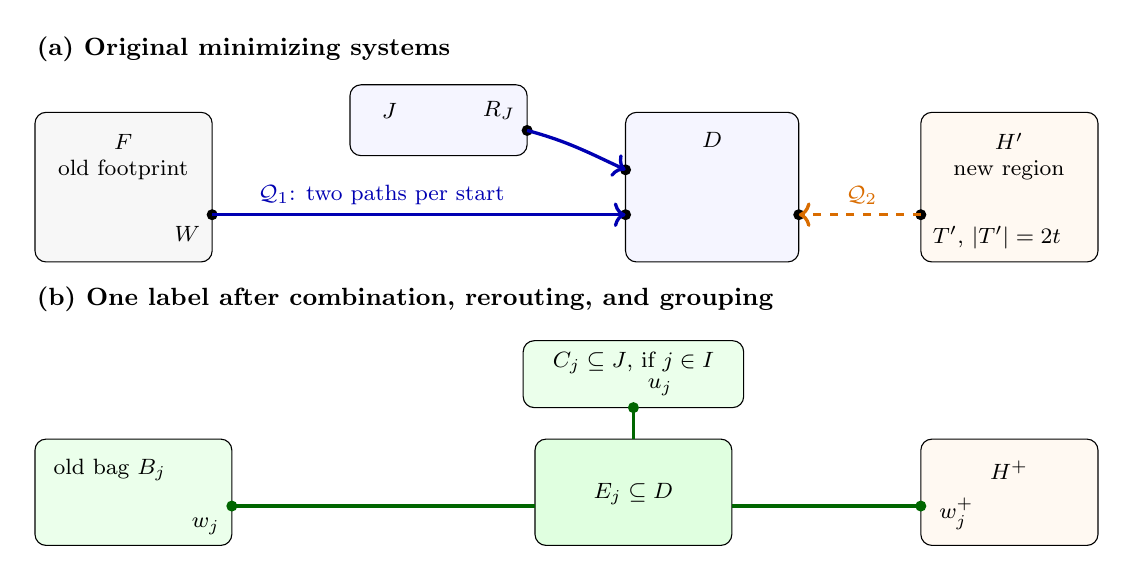
\begin{tikzpicture}[x=1cm,y=1cm,font=\footnotesize]
  \node[anchor=west,font=\small\bfseries] at (0,6.55)
    {(a) Original minimizing systems};
  \draw[rounded corners,fill=black!3] (0.1,3.85) rectangle (2.35,5.75);
  \node at (1.22,5.38) {\(F\)};
  \node at (1.22,5.02) {old footprint};
  \fill (2.35,4.45) circle (2pt);
  \node[below left] at (2.32,4.43) {\(W\)};

  \draw[rounded corners,fill=blue!4] (4.1,5.2) rectangle (6.35,6.1);
  \node at (4.6,5.77) {\(J\)};
  \fill (6.35,5.52) circle (2pt);
  \node[above left] at (6.32,5.53) {\(R_J\)};

  \draw[rounded corners,fill=blue!4] (7.6,3.85) rectangle (9.8,5.75);
  \node at (8.7,5.4) {\(D\)};
  \fill (7.6,4.45) circle (2pt);
  \fill (7.6,5.02) circle (2pt);
  \fill (9.8,4.45) circle (2pt);

  \draw[rounded corners,fill=orange!5] (11.35,3.85) rectangle (13.6,5.75);
  \node at (12.47,5.38) {\(H'\)};
  \node at (12.47,5.02) {new region};
  \fill (11.35,4.45) circle (2pt);
  \node[below right] at (11.38,4.43) {\(T'\), \(|T'|=2t\)};

  \draw[->,very thick,blue!70!black] (2.35,4.45) -- (7.6,4.45);
  \node[above,text=blue!70!black] at (4.5,4.45)
    {\(\mathcal Q_1\): two paths per start};
  \draw[->,very thick,blue!70!black]
    (6.35,5.52) to[out=-15,in=155] (7.6,5.02);
  \draw[->,very thick,dashed,orange!85!black]
    (11.35,4.45) -- (9.8,4.45);
  \node[above,text=orange!85!black] at (10.6,4.45)
    {\(\mathcal Q_2\)};

  \node[anchor=west,font=\small\bfseries] at (0,3.38)
    {(b) One label after combination, rerouting, and grouping};
  \draw[rounded corners,fill=green!8] (0.1,0.25) rectangle (2.6,1.6);
  \node at (1.05,1.21) {old bag \(B_j\)};
  \fill[green!40!black] (2.6,0.75) circle (2pt);
  \node[below left] at (2.57,0.72) {\(w_j\)};

  \draw[rounded corners,fill=green!12] (6.45,0.25) rectangle (8.95,1.6);
  \node at (7.7,0.9) {\(E_j\subseteq D\)};

  \draw[rounded corners,fill=green!8] (6.3,2.0) rectangle (9.1,2.85);
  \node at (7.7,2.57) {\(C_j\subseteq J\), if \(j\in I\)};
  \fill[green!40!black] (7.7,2.0) circle (2pt);
  \node[above right] at (7.76,2.03) {\(u_j\)};
  \draw[very thick,green!40!black] (7.7,2.0) -- (7.7,1.6);

  \draw[rounded corners,fill=orange!5] (11.35,0.25) rectangle (13.6,1.6);
  \node at (12.47,1.21) {\(H^+\)};
  \fill[green!40!black] (11.35,0.75) circle (2pt);
  \node[right] at (11.46,0.65) {\(w_j^+\)};
  \draw[very thick,green!40!black] (2.6,0.75) -- (6.45,0.75);
  \draw[very thick,green!40!black] (8.95,0.75) -- (11.35,0.75);
\end{tikzpicture}
\caption{A separability round, shown schematically.
The upper arrows represent families of paths; the two families may
intersect, and their entire vertex sets remain in the footprint.
Below, \(E_j\) joins label \(j\)'s path ends in \(D\).
The region \(H^+\) is obtained from \(H'\) by removing unused starts;
it meets the footprint exactly in the new tips \(W^+\).}
\label{fig:separability-round}
\end{figure}


Extend \(B_j\) by the two or three corresponding paths, by \(E_j\),
and by \(C_j\) when \(j\in I\). The resulting set \(B_j^+\) is
connected: its old bag contains \(w_j\); the paths join every
attached piece to \(E_j\); and it contains the new tip \(w_j^+\).
The sets \(B_j^+\) are pairwise disjoint. Indeed, the old bags
are disjoint and meet the added paths only at their own \(W\)-ends;
the paths are disjoint; the sets \(E_j\) are disjoint and meet paths
only at the designated terminals; and the bags \(C_j\) are
disjoint, lie outside \(F\cup D\), and meet paths only at their
own roots. All these sets lie in \(F^+\).
Old adjacencies persist because \(B_j\subseteq B_j^+\), and every
pair of labels in \(I\) gains an adjacency through its bags in
the district model.

It remains to check the next-region invariant. Exactly \(t\) vertices
were deleted from the \((K_0+1)t\)-connected
graph \(H'\), so \(H^+\) is \(K_0t\)-connected. By
\eqref{separate:new-region-list} and \eqref{separate:ch},
\[
 \ell(H^+)
 \ge r-\bigl(c_f+6(K_0+1)+1\bigr)t
 \ge r-c_ht.
\]
Equation~\eqref{separate:region-footprint} gives
\[
 V(H^+)\cap F^+=W^+.
\]
Thus \(F^+,H^+,W^+\), and the bags \(B_j^+\) restore every
invariant for the next round.

After all \(R_t\) rounds, every pair of labels has an adjacency.
The \(t\) disjoint connected label bags therefore form a \(K_t\)
model in \(G\), contradicting \(h(G)<t\).
This proves Lemma~\ref{lem:separability}.
\end{proof}

\section{Recursive weaving and the universal bound}\label{sec:recursion}

The recursive use of woven districts follows the framework of
Postle \cite[Section~6]{Postle2020} and Delcourt and Postle
\cite[Section~7]{DelcourtPostle2021}. We now use separability to replace
the successive small steps of the preceding section by a recursion with
a fixed shrinkage factor.

\begin{theorem}\label{thm:recursive-woven}
There are absolute positive integers $K,Q$ such that, for every integer
$a\ge1$, every $Ka$-connected graph $P$ with $\ell(P)\ge Qa$ is
$(a,3a)$-woven.
\end{theorem}
\begin{proof}
The main inductive step concerns $h(P)<64a$ and sufficiently large $a$.
It separates the paths for prescribed pairs from the clique-model
construction. Give each root and each end of a noncoincident pair its
own neighboring proxy outside the original terminal set, with all proxies
distinct, and delete the original terminals. Choose a minimum-total-length
system of two paths per proxy to a small highly connected district $D$.
Deleting the proxies, $D$, and these paths costs only $O(a)$ in list
chromatic number. We can therefore extract a highly connected region
$H'$ disjoint from the first path system. Further connections
from $H'$ to $D$ and Lemma~\ref{lem:combine} produce disjoint paths from
all proxies and from a set $W$ of $a$ vertices of $H'$ to $D$, meeting
$H'$ only at $W$. It then suffices to build a clique model rooted at $W$
inside $H'$: grouping the path ends in $D$ attaches the model to the
root proxies and completes the prescribed pair paths.

For this internal model, divide the labels of $W$ into three blocks.
Separability and connectivity extraction supply three disjoint
districts for recursive calls, one for each pair of blocks. A call
needs at most $2\lceil a/3\rceil$ roots. Each label receives two bags
to be joined to its vertex of $W$. The $2a$ joining paths may pass through
the recursive districts; wovenness lets us reroute them while constructing
the child models, keeping the retained bags disjoint from the paths
except at their designated roots. Every pair of labels shares a district
and hence receives an adjacency.

We specify the order of the constants first. Fix all constants in the
preceding sections, including $L,C_*,B_*,K_0,D_{K_0}$, the deletion
constants $c_d$, and the separability constant $S$. Choose an integer
$K\ge100$ such that
\begin{equation}\label{recursive:K}
 K-14>128D_{K_0}.
\end{equation}
Choose an absolute integer $a_0\ge24$ so large that all sufficiently-large
parameter conclusions used below hold with $t=64a$ whenever $a>a_0$.
Enlarge $a_0$ if necessary so that
\begin{equation}\label{recursive:shrink}
 a'=2\lceil a/3\rceil\le3a/4\qquad(a>a_0),
\end{equation}
and $t^{1.06}+7a\le t^{11/10}$ for $t=64a$, $a>a_0$.
All these requirements involve only constants already fixed, and none
involves $Q$. Finally choose an integer $Q$ satisfying
\begin{align}
 Q/4&>10+64(c_{42}+6K_0+2S)+(9/2)K,
       \label{recursive:Q-induction}\\
 Q&>10+64(c_{42}+6K_0+3S),
       \label{recursive:Q-separation}\\
 Q&>128C_*\log(128a_0)+1.
       \label{recursive:Q-base}
\end{align}
We prove the assertion by strong induction on $a$.

\paragraph{Separating the terminal roles.}
Fix $a$ distinct roots and at most $3a$ pairs as in
Definition~\ref{def:woven}. Let $Z_0$ be their union, so $|Z_0|\le7a$.
For each root, and for each end of each noncoincident pair, choose a
neighbor outside $Z_0$ as its \emph{proxy}. All proxies are distinct,
even for different roles of the same original vertex. This is possible
greedily because $\delta(P)\ge Ka$ and fewer than $14a$ vertices are
forbidden at any choice. Coincident pairs will ultimately use trivial
paths at their original vertices and need no proxies.

Put $G=P-Z_0$ and let $Z$ be the proxy set. Then
\begin{equation}\label{recursive:proxy-bounds}
 a\le|Z|\le7a,\qquad
 G\text{ is }(K-7)a\text{-connected},\qquad
 \ell(G)\ge Qa-7a.
\end{equation}
It suffices to find in $G$ a clique model rooted at the root proxies and
paths for the other proxy pairs, with all model bags and all these paths
pairwise disjoint. Adding the proxy edges and the original vertices then
restores precisely the root--path coincidences allowed by wovenness.
Different prescribed pairs have no common original endpoint; a
coincident pair at a root meets only that root's expanded bag.

\paragraph{A large minor and the finite base range.}
Set $t=64a$. If $h(P)\ge t$, delete from a $K_t$ model every bag meeting
$Z_0$. This leaves a $K_{57a}$ model in $G$. Since
$57a\ge4|Z|$ and $(K-7)a\ge2|Z|$, Lemma~\ref{lem:rooting} gives a
clique model rooted at all of $Z$. Retain the root-proxy bags. For each
other proxy pair, a path through its two bags and an edge between them
joins the pair. These paths and the retained bags are disjoint because
all proxies and their bags are distinct. This proves the required
conclusion in the large-minor case, for every $a$.

Suppose $h(P)<64a$. Lemma~\ref{lem:coarse-density} gives
\[
 \ell(P)\le128C_*a\log(128a)+1.
\]
For $1\le a\le a_0$ this is strictly less than $Qa$ by
\eqref{recursive:Q-base}. Thus the minor-free case is impossible
throughout the base range. We may henceforth assume $a>a_0$.

\paragraph{A junction district and a fresh region.}
Every vertex of $G-Z$ has degree at least $(K-14)a$, which is greater
than $2D_{K_0}t$ by \eqref{recursive:K}. In particular this graph is
nonempty and has density greater than $D_{K_0}t$. Apply
Lemma~\ref{lem:district} to find a $K_0t$-connected district
$D\subseteq G-Z$ with $|V(D)|\le t^{1.06}$.

The connectivity of $G$ and the order of $D$ permit two paths per proxy
from $Z$ to distinct vertices of $D$, with only the prescribed repeated
starts in common, by Lemma~\ref{lem:double-packing}. Choose such a system
$\mathcal Q_1$ of minimum total length in $G$. It has at most $14a$ paths.
Put
\[
 X=Z\cup V(D),\qquad Y=V(\mathcal Q_1)\setminus X.
\]
We have $|X|\le t^{11/10}$ by the choice of $a_0$.
Lemma~\ref{lem:path-minimization} gives $28a$-degeneracy of $G[Y]$ and
at most $42a$ neighbors in $Y$ for every vertex outside $X\cup Y$.
These bounds are at most $42t$, so Lemma~\ref{lem:additive-deletion}
with parameter $42$ gives
\begin{equation}\label{recursive:after-paths}
 \ell(G-X-Y)\ge Qa-7a-c_{42}t.
\end{equation}
By \eqref{recursive:Q-separation} the right-hand side exceeds $6K_0t$.
Lemma~\ref{lem:list-extraction} therefore supplies a $K_0t$-connected
induced subgraph $H'\subseteq G-X-Y$ such that
\begin{equation}\label{recursive:Hprime}
 \ell(H')\ge Qa-7a-(c_{42}+6K_0)t.
\end{equation}

In $G-Z$, the sets $H'$ and $D$ have order greater than $K_0t$, and the
connectivity is at least $(K-14)a>2a$. Hence there are $2a$ disjoint
$H'$-to-$D$ paths. Truncate them at their last visit to $H'$ and their
first subsequent visit to $D$, so they have no internal vertex in either
set. They avoid $Z$. Lemma~\ref{lem:combine}, applied to these paths and
$\mathcal Q_1$, gives disjoint paths to $D$ from all proxies in $Z$ and
from a set $W$ of $a$ distinct vertices of $H'$. These paths meet $H'$ and
$D$ only at their appropriate ends.

It is now enough to construct a clique model rooted at $W$ entirely
inside $H'$. Indeed, in $D$ group the terminal ends of the outside paths
as follows: pair each root proxy with a different member of $W$, and
pair the other proxies as prescribed. There are at most $|Z|+a\le8a$
terminals, so Theorem~\ref{thm:grouping} applies because
$K_0t\ge8\gamma a$. These disjoint groups and the outside paths attach
the rooted model to the root proxies and supply all other required
paths. The model inside $H'$ has no unwanted intersection with the
outside paths, since their only vertices in $H'$ are precisely $W$.

\paragraph{Three recursive districts.}
For each $w\in W$ choose two neighbors in $H'-W$, all $2a$ choices
distinct. Minimum degree at least $K_0t$ permits this greedy choice.
Let $N$ be their set and put $H''=H'-W-N$. Then
\begin{equation}\label{recursive:r0}
 \ell(H'')\ge r_0:=Qa-10a-(c_{42}+6K_0)t.
\end{equation}
Equation~\eqref{recursive:Q-separation} gives $r_0>3St$.
Apply Lemma~\ref{lem:separability} to $H''$, and then to one of the two
resulting subgraphs. The first application is legal because
$\ell(H'')\ge r_0>2St$. Each of its subgraphs has list chromatic number
at least $r_0-St>2St$, making the second application legal as well.
We obtain three disjoint subgraphs each of list chromatic number at
least $r_0-2St$.

Take $a'=2\lceil a/3\rceil$. After the loss of $2St$ to separability,
each subgraph must still pay $6Ka'$ for connectivity extraction and
retain $Qa'$ for the recursive call. If
$A=10+64(c_{42}+6K_0+2S)$, then
\begin{align*}
 r_0-2St-6Ka'-Qa'
 &=Q(a-a')-Aa-6Ka'\\
 &\ge\bigl[Q/4-A-(9/2)K\bigr]a>0
\end{align*}
by \eqref{recursive:shrink} and \eqref{recursive:Q-induction}.
In particular $r_0-2St>6Ka'$, and list extraction in each subgraph
produces disjoint $Ka'$-connected induced districts $J_1,J_2,J_3$
with list chromatic number at least $Qa'$. Since $a'<a$, induction
makes each district $(a',3a')$-woven.

Partition the labels of $W$ into three nonempty blocks $B_1,B_2,B_3$,
each of size at most $\lceil a/3\rceil$. Assign one district to each
pair of blocks, relabeling them $J_{12},J_{13},J_{23}$ accordingly.
In its district, designate a distinct root for each
label of the corresponding two blocks, and add arbitrary distinct
padding roots to bring the total to $a'$. The districts have enough
vertices for this choice. Every label has exactly two designated roots,
in different districts; every pair of labels occurs together in at
least one district, including two labels in the same block; see
Figure~\ref{fig:three-districts}.

\begin{figure}[tb]
\centering
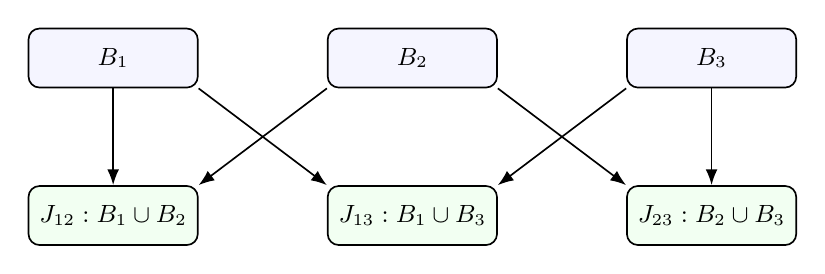
\begin{tikzpicture}[font=\small,
 block/.style={draw,rounded corners,minimum width=2.15cm,minimum height=.75cm,fill=blue!4},
 district/.style={draw,rounded corners,minimum width=2.15cm,minimum height=.75cm,fill=green!5},
 every path/.style={line width=.6pt}]
\node[block] (b1) at (0,2) {$B_1$};
\node[block] (b2) at (3.8,2) {$B_2$};
\node[block] (b3) at (7.6,2) {$B_3$};
\node[district] (j12) at (0,0) {$J_{12}: B_1\cup B_2$};
\node[district] (j13) at (3.8,0) {$J_{13}: B_1\cup B_3$};
\node[district] (j23) at (7.6,0) {$J_{23}: B_2\cup B_3$};
\draw[-{Latex[length=2mm]}] (b1.south) -- (j12.north);
\draw[-{Latex[length=2mm]}] (b1.south east) -- (j13.north west);
\draw[-{Latex[length=2mm]}] (b2.south west) -- (j12.north east);
\draw[-{Latex[length=2mm]}] (b2.south east) -- (j23.north west);
\draw[-{Latex[length=2mm]}] (b3.south west) -- (j13.north east);
\draw[-{Latex[length=2mm]}] (b3.south) -- (j23.north);
\end{tikzpicture}

\caption{The three recursive districts. The blocks $B_1,B_2,B_3$ partition
the labels, and a label has one designated root in each of the two
districts receiving its block. Arrows indicate label assignments, not
graph edges. Every pair of labels is represented together in a district.}
\label{fig:three-districts}
\end{figure}

Inside $H'-W$, join the two chosen neighbors of each $w$ to its two
designated roots, respectively, using disjoint paths. This is an
application of Theorem~\ref{thm:grouping} to $4a$ distinct terminals:
the neighbors lie in $N$, while the districts were chosen in $H''$
and hence avoid $N$. The connectivity is at least $K_0t-a\ge4\gamma a$.
There are $2a$ paths. Apply Lemma~\ref{lem:rerouting} successively in the
three districts to incorporate their rooted clique models while
retaining these path ends. Each district has sufficient weaving
capacity, since
\[
 2a\le3a'=6\lceil a/3\rceil.
\]
Discard all padding bags. Each designated root remains an endpoint
of its path; the retained bags meet the rerouted paths only at their
own designated roots. Since the districts are disjoint, later rerouting
does not introduce an intersection in a previously retained bag.

For each $w$, unite its two designated bags with their respective paths,
the two edges to $w$, and $w$ itself. The resulting $a$ sets are connected
and disjoint, rooted at $W$. Two labels have an edge between their sets
because they occur together in one of the district clique models.
This constructs the required rooted $K_a$ model inside $H'$ and
completes the induction.
\end{proof}

\begin{proof}[Proof of Theorem~\ref{thm:main}]
Let $K,Q$ be as in Theorem~\ref{thm:recursive-woven}. We first show that,
for every integer $t\ge2$,
\begin{equation}\label{recursive:final-minor-free}
 h(G)<t\quad\Longrightarrow\quad\ell(G)\le(Q+6K)t.
\end{equation}
Otherwise Lemma~\ref{lem:list-extraction}, with connectivity parameter
$Kt$, gives a $Kt$-connected induced subgraph $P$ with
$\ell(P)\ge\ell(G)-6Kt>Qt$. Theorem~\ref{thm:recursive-woven} makes
$P$ $(t,3t)$-woven. Its order is greater than $Kt\ge t$, so we may choose
$t$ roots and no pairs. Wovenness then supplies a $K_t$ model,
contradicting $h(G)<t$.

For a nonempty graph, $h(G)\ge1$. Taking $t=h(G)+1\le2h(G)$ in
\eqref{recursive:final-minor-free} proves
\[
 \ell(G)\le2(Q+6K)h(G).
\]
Thus the absolute integer $C=2(Q+6K)$ has all the claimed uniformity.
The finite base range was covered before the induction began, so no
small-parameter exception remains.
\end{proof}

\bibliographystyle{plainnat}
\bibliography{references}
\end{document}
